\documentclass[11pt,letterpaper]{article}

% Packages
\usepackage[utf8]{inputenc}
\usepackage[margin=1in]{geometry}
\usepackage{amsmath,amssymb}
\usepackage{textgreek}  % For Ω, Δ
\usepackage{graphicx}
\usepackage{booktabs}
\usepackage{hyperref}
\usepackage{xcolor}
\usepackage{listings}
\usepackage{caption}
\usepackage{subcaption}

% Metadata
\title{Self-Play Calibration of Heuristic Agents for Mexican Train Under Competing Objectives}

\author{
  Digital Defiance \\
  \texttt{https://github.com/digitaldefiance/warp12}
}

\date{\today}

\begin{document}

\maketitle



\begin{abstract}
Mexican Train dominoes is commonly played under two incompatible victory conditions: \textbf{points} (lowest pip total when the round ends) and \textbf{go-out} (first player to empty their hand). This paper describes the development, calibration, and empirical validation of AI agents for both objectives in Warp 12, an open-source Mexican Train implementation. We introduce the \textbf{Tactical Effectiveness Index (TEI)}, a dual-track OpenSkill-based rating system with gamified grade display, anchored to fixed AI reference tiers.

Empirical results from thousands of self-play games show that \textbf{skill ordering is stable under the points objective} (consistent rating gaps between tiers), while \textbf{go-out exhibits higher variance} and compressed skill gaps. We demonstrate that search algorithms provide different advantages depending on context: expectimax wins in 2-player points (64\% vs heuristics), while ISMCTS excels in 4+ player go-out (31\% vs 23\% baseline). 

A comprehensive 19,000-game empirical study across 38 configurations (4 Warp factors $\times$ 2--18 players) reveals that \textbf{skill expression increases with both tile set size and player count}, contradicting the intuition that larger games devolve into luck. We show that Warp factor 12 (double-twelve dominoes) is the empirically optimal choice for competitive rating, exhibiting the highest sensitivity to player skill.

Finally, we report on \textbf{Class $\Omega$}, a neural self-play agent that achieves parity with heuristic baselines in small games and outperforms in large fleets, demonstrating that pure self-play can produce competitive agents without hand-crafted heuristics. All code, data, and reproduction scripts are available as open source.
\end{abstract}

\section{Introduction}

\subsection{Mexican Train Dominoes}

Mexican Train is a popular multi-player domino game typically played with a double-twelve set (91 tiles with pips ranging from 0 to 12). Players build linear sequences called \textit{trains} from a central \textit{engine} (starting double), attempting to minimize their hand's pip count. The game features both private trains (one per player) and a shared public train (the ``Mexican Train'' or Neutral Zone), creating strategic tension between building one's own position and blocking opponents.

Unlike classic domino games with a single win condition, Mexican Train is commonly played under two incompatible objectives:
\begin{itemize}
\item \textbf{Points campaign:} Play continues for multiple rounds (descending from engine double-12 down to double-0). After each round, players accumulate penalty points equal to the pips remaining in their hand. Lowest cumulative score after all rounds wins.
\item \textbf{Go-out:} The first player to empty their hand wins immediately, ending the round.
\end{itemize}

These objectives create fundamentally different strategic games on the same rules engine: points rewards consistent pip minimization and flexible play across many turns, while go-out rewards tempo, connectivity, and race dynamics.

\subsection{Warp 12: Terminology and Presentation}

This paper describes work conducted in the context of Warp 12, an open-source Mexican Train implementation with a Star Trek-themed presentation layer. Throughout this paper, we use \textbf{standard Mexican Train terminology} in formal discussion, but introduce Warp 12's thematic terminology where relevant to implementation details. The table below provides a complete mapping.

\begin{table}[h]
\centering
\caption{Warp 12 terminology mapped to Mexican Train equivalents}
\label{tab:terminology}
\begin{tabular}{@{}lll@{}}
\toprule
\textbf{Mexican Train} & \textbf{Warp 12} & \textbf{Technical} \\
\midrule
\multicolumn{3}{@{}l}{\textit{Game Elements}} \\
Domino / tile & Navigational Coordinate & \texttt{Coordinate} \\
Engine (starting double) & Spacedock & \texttt{engine} \\
Player's private train & Warp Trail & \texttt{ownTrail} \\
Mexican Train (public) & Neutral Zone & \texttt{neutralZone} \\
Train marker / forced play & Distress Beacon & \texttt{beacon} / \texttt{shieldsDown} \\
Unsatisfied double & Red Alert & \texttt{redAlert} \\
Draw pile & Uncharted Sectors & \texttt{pile} \\
\midrule
\multicolumn{3}{@{}l}{\textit{Players and Rating}} \\
Player & Captain & \texttt{PlayerId} \\
Skill rating & TEI & \texttt{tei} (integer) \\
Game table & Sector / Fleet & \texttt{game} \\
\midrule
\multicolumn{3}{@{}l}{\textit{AI Tiers}} \\
Easy AI & Class IV (Ensign) & \texttt{ensign} \\
Medium AI & Class III (Lieutenant) & \texttt{lieutenant} \\
Hard AI & Class II (Commander) & \texttt{commander} \\
Expert (human only) & Class I & TEI $\geq$ 1450 \\
\bottomrule
\end{tabular}
\end{table}

\textbf{Warp factors} refer to the maximum pip value in the domino set: Warp 9 (W9) uses double-nine tiles (55 tiles total), Warp 12 (W12) uses double-twelve (91 tiles), etc. Throughout this paper, we use compact notation \textbf{WX/Yp} to denote configurations: W12/4p means Warp factor 12 (double-twelve) with 4 players. This paper focuses on W12 as the primary rated configuration, with analysis of W9, W15, and W18 in Section~8.

\subsection{Motivation}

Despite Mexican Train's popularity, it remains under-studied in the game AI literature compared to chess, Go, or poker. Several challenges make it interesting for AI research:

\begin{itemize}
\item \textbf{Imperfect information:} Opponent hands and draw pile order are hidden, requiring belief-state reasoning rather than perfect-information tree search.
\item \textbf{Multi-player dynamics:} Unlike 2-player zero-sum games, Mexican Train typically involves 3--8 players with complex coalition and blocking incentives.
\item \textbf{Dual objectives:} The same rule set produces two strategically distinct games depending on win condition.
\item \textbf{Stochastic elements:} Random draws from the pile, variable starting hands, and opponent action uncertainty all contribute to outcome variance.
\end{itemize}

For online play, these challenges create practical design questions: How do we measure player skill fairly? How do we provide appropriately challenging AI opponents? How do we ensure coaching tools don't contaminate competitive ratings?

\subsection{Contributions}

This paper makes the following contributions:

\begin{enumerate}
\item \textbf{Dual-track TEI rating system} --- We describe an OpenSkill-based rating with independent tracks for points and go-out objectives, anchored to fixed AI reference tiers rather than floating human populations. The system uses Bayesian inference with $\mu \pm \sigma$ skill estimates and presents ratings as gamified grades (E/V/C/I/P + 0-99 score).

\item \textbf{Self-play calibration methodology} --- We present a systematic approach to validating AI skill levels through tier-vs-tier matrices, symmetric seating tests, and multi-player focus matchups.

\item \textbf{Empirical objective comparison} --- Through thousands of self-play games, we demonstrate that points calibrates cleanly with consistent rating gaps between tiers, while go-out exhibits compression and higher variance due to its racing mechanics.

\item \textbf{Search algorithm analysis} --- We show that different search methods (expectimax, ISMCTS) provide advantages in different contexts: expectimax excels in 2-player points (64\% win rate), while ISMCTS works better in 4+ player go-out (31\% vs 23\% baseline).

\item \textbf{Luck vs skill across configurations} --- A 19,000-game empirical study across 38 configurations reveals that skill expression increases with both tile set size and player count, with Warp 12 (double-twelve) emerging as the empirically optimal choice for competitive rating.

\item \textbf{Module balance and competitive integrity} --- Pending empirical validation of optional game mechanics and their impact on skill expression in competitive play.

\item \textbf{Neural self-play agent (Class $\Omega$)} --- We demonstrate that a pure self-play neural policy can achieve competitive performance (parity in small games, advantages in large fleets) without hand-crafted heuristics, and discuss the challenges of mapping training performance to appropriate rating anchors.

\item \textbf{Open-source implementation} --- All code, data, and reproduction scripts are available through the warp12-engine package and associated repositories.
\end{enumerate}

\section{Related Work}

This section briefly surveys prior work in domino game AI, game AI paradigms relevant to Mexican Train, and skill rating systems. We identify the specific gap this work fills.

\subsection{Domino and Tile Games}

Domino games have received limited attention in the game AI literature compared to board games like chess and Go or card games like poker. Most prior work focuses on simpler variants like straight dominoes or block dominoes, which lack Mexican Train's multi-player train mechanics and dual objectives. The DoubleEighteen rendering library~\cite{doubleighteen2024} provides visualization for domino games but does not include AI agents. To our knowledge, this is the first published calibration study of AI agents for Mexican Train specifically.

\subsection{Game AI Paradigms}

Several AI approaches are relevant to imperfect-information multi-player games like Mexican Train:

\textbf{Heuristic policies:} Hand-crafted evaluation functions and decision rules remain competitive in many domains, especially where interpretability matters for player trust and coaching features. Our Class IV--II agents follow this tradition with weighted heuristics for pip dumping, trail pressure, and blocking.

\textbf{Monte Carlo Tree Search (MCTS):} MCTS and its variants~\cite{browne2012mcts} have achieved strong results in perfect-information games (Go, Hex) and some imperfect-information settings. Information Set MCTS (ISMCTS)~\cite{cowling2012ismcts} handles hidden information by sampling determinizations and maintaining search trees over information sets rather than individual states. We use ISMCTS for our Fleet Admiral and Class $\Omega$+ search backends.

\textbf{Deep reinforcement learning and self-play:} The AlphaZero family~\cite{silver2017alphazero,silver2018alphazero} demonstrated that pure self-play with neural networks can surpass human expertise in chess, Go, and shogi. However, these successes required massive computational resources and perfect information. Our Class $\Omega$ agent represents a more modest self-play approach suitable for imperfect-information games with limited training compute.

\textbf{Counterfactual regret minimization:} CFR and its variants have achieved superhuman performance in poker~\cite{bowling2015heads}, another imperfect-information game. However, CFR typically requires extensive offline precomputation and works best in 2-player zero-sum settings, making it less applicable to multi-player cooperative-competitive games like Mexican Train.

\subsection{Skill Rating Systems}

Several rating systems are widely used in competitive games:

\textbf{Elo rating~\cite{elo1978rating}:} Originally developed for chess, Elo computes expected win probabilities based on rating differences and updates ratings based on actual outcomes. It assumes transitive skill relationships and works best for 2-player zero-sum games.

\textbf{Glicko~\cite{glickman1999glicko}:} Extends Elo by modeling rating uncertainty (RD), allowing ratings to drift during inactivity periods and providing confidence intervals.

\textbf{TrueSkill~\cite{herbrich2006trueskill}:} Microsoft's rating system extends to multi-player and team games using Bayesian inference. It models each player's skill as a Gaussian distribution and updates beliefs after each match.

\textbf{OpenSkill:} An open-source implementation of rating systems inspired by TrueSkill and Weng-Lin ranking~\cite{wenglin2011}, designed for multi-player and team-based games. Like TrueSkill, it uses Gaussian skill models with mean ($\mu$) and standard deviation ($\sigma$) parameters, updated through Bayesian inference. We adopt OpenSkill as the foundation for TEI due to its multi-player support, open implementation, and flexible team rating capabilities.

Most online game platforms (Chess.com, Lichess, etc.) use Elo or Glicko variants. Some platforms that offer AI opponents (e.g., Lichess's Stockfish bots) provide fixed rating estimates for bot difficulty levels, similar to our TEI anchor approach. However, we are unaware of prior work that systematically calibrates and validates AI skill tiers through self-play specifically for the purpose of providing stable rating anchors.

\subsection{Contribution Relative to Prior Work}

This work makes several novel contributions relative to the existing literature:

\begin{enumerate}
\item \textbf{Dual-objective calibration:} We systematically compare points and go-out objectives on the same rules engine, showing empirically that they require different strategic optimization and exhibit different skill/variance tradeoffs.

\item \textbf{Fixed AI reference anchors:} Rather than deriving ratings entirely from human populations (which can drift over time), we anchor rating bands to validated AI tiers with measured performance characteristics.

\item \textbf{Multi-player self-play methodology:} Most game AI calibration focuses on 2-player matchups. We include 3--8 player configurations and focus matchups (one strong player vs multiple weaker opponents) to validate skill expression in realistic play scenarios.

\item \textbf{Luck vs skill empirics:} The 19,000-game study across 38 configurations provides the first systematic measurement of how tile set size and player count affect skill expression in domino games.

\item \textbf{Open-source implementation:} All code (rules engine, AI agents, calibration scripts) and data are publicly available for reproduction and extension.
\end{enumerate}

\section{Game Model and Rules Engine}

\subsection{Core Mexican Train Rules}

Mexican Train follows standard multi-trail domino game mechanics:

\begin{enumerate}
\item \textbf{Setup:} All players draw a fixed hand size (typically 15 tiles for 2--4 players, fewer for larger games). The engine double (e.g., 12-12 for Warp 12) is placed in the center. Remaining tiles form the draw pile.

\item \textbf{Turn structure:} On each turn, a player must play one tile that matches the open end of any available train (their own, another player's with a marker, or the public Mexican Train). If unable to play, they draw one tile from the pile and may play it immediately if legal.

\item \textbf{Doubles:} When a double is played, it must be ``satisfied'' (another tile played on it) before anyone can play elsewhere. This creates a \textit{Red Alert} state that forces immediate resolution.

\item \textbf{Train markers:} When a player cannot play on their turn, they place a marker on their train, making it public for one round. In Warp 12 terminology, this is called a \textit{Distress Beacon} and the state is \textit{Shields Down}.

\item \textbf{Mexican Train:} The public train is always available to all players, providing a release valve when private trains are blocked.

\item \textbf{Round end:} A round ends when a player empties their hand (go-out objective) or when the pile is exhausted and no legal plays remain (points objective).
\end{enumerate}

\subsection{Implementation as State Machine}

Our implementation models the game as an immutable state machine with pure functions:

\begin{itemize}
\item \textbf{State:} Readonly data structures (\texttt{GameState}, \texttt{RoundState}, \texttt{TableState}) containing all game information: player hands, visible tiles, pile size, train states, alert conditions.

\item \textbf{Actions:} Typed events (\texttt{PlayAction}, \texttt{DrawAction}, etc.) representing legal moves.

\item \textbf{Transitions:} Pure function \texttt{applyAction(state, action) -> newState} implements all rules.

\item \textbf{Legal moves:} Function \texttt{getLegalMoves(state, playerId) -> Action[]} computes all valid plays for the current state.
\end{itemize}

This design ensures that AI agents, human players, and replay validation all use identical game logic. No special-case code paths exist for AI vs human play.

\subsection{House Rules and Modules}

Beyond core rules, Mexican Train has many common variants. Warp 12 implements these as runtime configuration rather than hard-coded variants:

\textbf{House rules} (boolean toggles):
\begin{itemize}
\item \texttt{requireOwnTrailFirst}: Must play on own train before playing elsewhere
\item \texttt{neutralZoneAfterAllTrails}: Mexican Train only available after personal train started
\item \texttt{dropToImpulse}: ``Uno''-style announce requirement when down to one tile
\end{itemize}

\textbf{Modules} (optional mechanics):
\begin{itemize}
\item \textbf{Alpha (Continuum):} Special rules for 0-0 tile (Q-gamble mechanic)
\item \textbf{Beta (Salamander Penalty):} Pip penalty for holding double-zero at round end
\item \textbf{Gamma (Sensor Grid):} Tiles visible for potential recycling
\item \textbf{Delta (Hot Potato):} Hazard marker transfers on Neutral Zone play (+5 per pass while holding)
\item \textbf{Theta (Longest Trail):} Bonus for longest personal train with chain-draw mechanic
\item \textbf{Iota (Double Down):} Playing a double forces next player to draw 2 tiles
\item \textbf{Kappa (Temporal Inversion):} Odd rounds score normally, even rounds invert (highest wins)
\end{itemize}

All modules affect legal move generation and scoring through the same \texttt{applyAction} code path, ensuring AI agents see exactly the same game mechanics as human players.

\subsection{Information Structure and Game Complexity}

Mexican Train is an \textbf{imperfect information game}:

\begin{itemize}
\item \textbf{Public information:} All played tiles on trains, player hand counts, draw pile size, train marker positions, active Red Alert doubles
\item \textbf{Hidden information:} Contents of opponent hands, order of tiles in draw pile
\end{itemize}

This differs fundamentally from perfect-information games like chess or Go, where optimal play can theoretically be computed through exhaustive search. In Mexican Train:

\begin{enumerate}
\item \textbf{Belief states:} Agents must reason about probability distributions over possible opponent hands and pile orderings, not a single deterministic state.

\item \textbf{Determinization:} One common approach samples possible hidden states consistent with observations, then searches forward in each determinized world. However, this can lead to strategy fusion~\cite{frank1996determinization} where different opponent hand distributions should lead to different plays.

\item \textbf{Information set search:} Methods like Information Set Monte Carlo Tree Search (ISMCTS)~\cite{cowling2012ismcts} explicitly handle information sets, avoiding some determinization pitfalls.
\end{enumerate}

The combination of hidden information, multi-player dynamics, and stochastic draws makes Mexican Train significantly more complex than its simple rules suggest, and prevents the existence of a "solved" optimal strategy comparable to checkers or Connect Four.

\subsection{Two Objectives as Two Different Games}

The choice of victory condition fundamentally changes optimal strategy:

\begin{table}[h]
\centering
\small
\begin{tabular}{@{}lll@{}}
\toprule
\textbf{Dimension} & \textbf{Points} & \textbf{Go-out} \\
\midrule
Win condition & Lowest pips at round end & First empty hand \\
Horizon & Multi-round campaign (1--13) & Often single-round race \\
Core skill & Pip shedding, blocking, flexibility & Tempo, connectivity, mayhem \\
Variance & Lower & Higher \\
Search benefit & Modest at 2p; expectimax depth 4 $\sim$64\% & Helpful at 2p; ISMCTS $\sim$31\% /4p \\
Reference TEI spacing & 200 pts / tier & 250 pts / tier \\
\bottomrule
\end{tabular}
\caption{Strategic differences between points and go-out objectives}
\label{tab:objectives}
\end{table}

In the \textbf{points} objective, players accumulate penalty points over 13 rounds, rewarding consistent pip minimization and defensive blocking. The multi-round horizon allows recovery from bad draws and rewards strategic flexibility.

In the \textbf{go-out} objective, the first player to empty their hand wins immediately. This creates race dynamics where tempo and hand connectivity matter more than pip values. A player holding three 12-12 doubles might still win if they can chain them quickly.

Figure~\ref{fig:points-vs-goout} shows empirically that these objectives lead to measurably different strategic landscapes, with go-out exhibiting compressed skill gaps and higher outcome variance.

\begin{figure}[htbp]
\centering
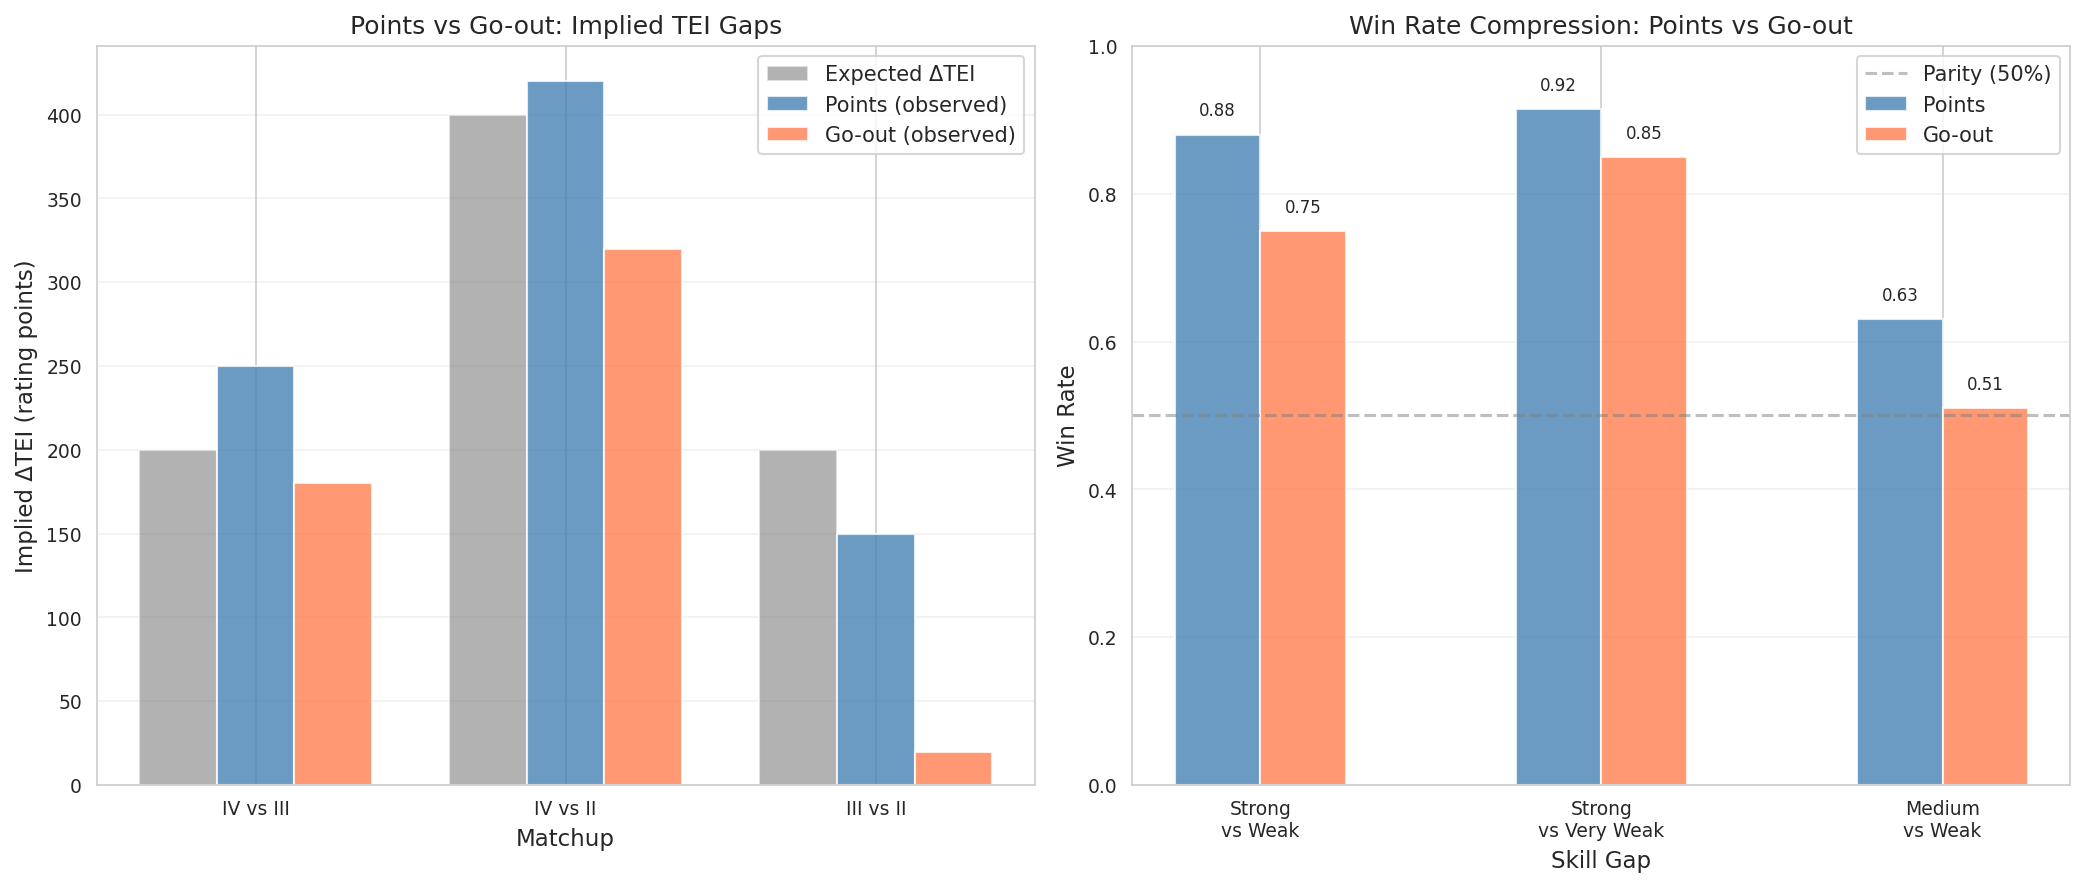
\includegraphics[width=0.9\textwidth]{../tools/nn/figures/figure10-points-vs-goout.png}
\caption{Points vs go-out strategic divergence. Left: Implied ΔTEI from observed win rates shows go-out compression. Right: Win rate distributions demonstrate that go-out behaves like a stochastic race (ordering survives, magnitudes compress).}
\label{fig:points-vs-goout}
\end{figure}

\section{Agent Architecture}

\begin{figure}[htbp]
\centering
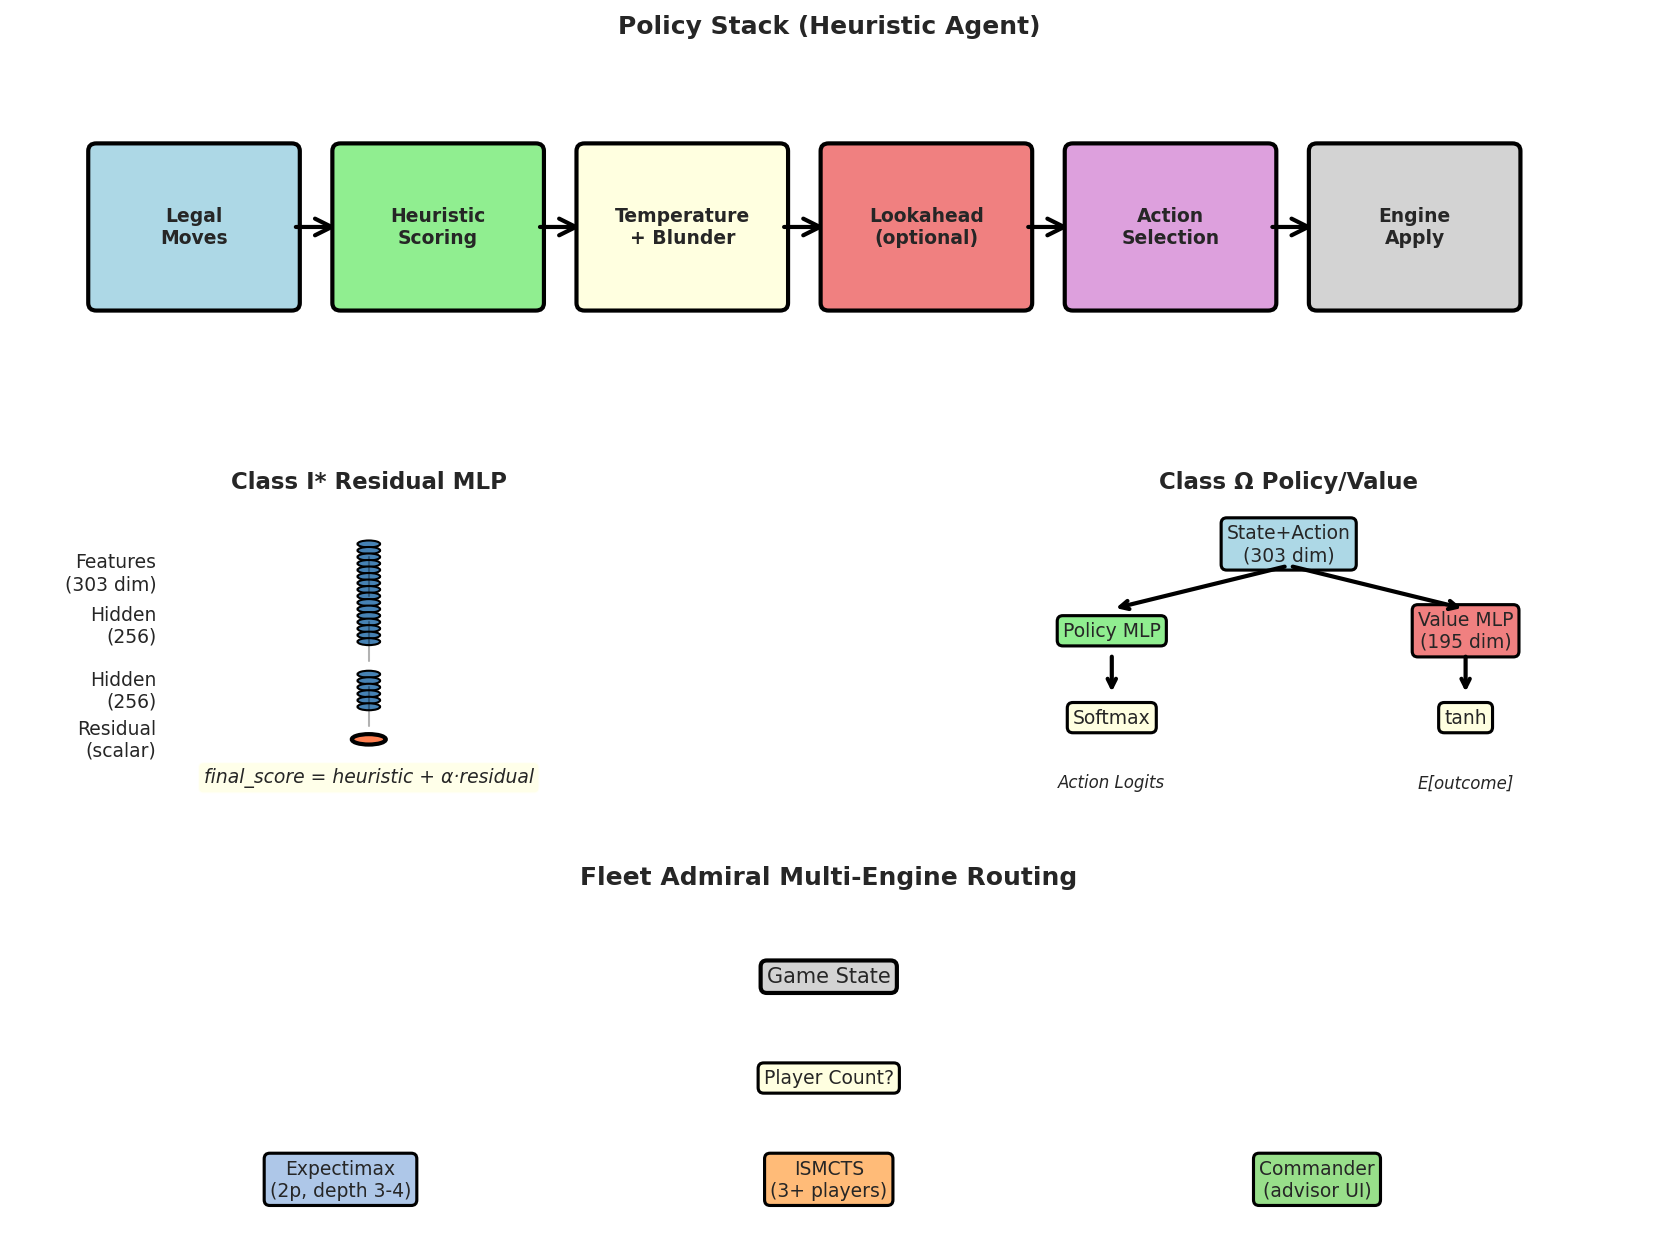
\includegraphics[width=0.95\textwidth]{../tools/nn/figures/figure9-architectures.png}
\caption{Agent architecture overview. Top: Heuristic policy stack (candidate generation through action selection). Middle-left: Class I* residual MLP adds learned correction to heuristics. Middle-right: Class Ω standalone policy/value heads (no heuristics). Bottom: Fleet Admiral multi-engine routing by player count.}
\label{fig:architectures}
\end{figure}

\subsection{Policy Stack}
Candidate generation from legal moves + special actions. Weighted heuristic scoring + temperature + blunder rate. Optional determinized lookahead: sample hidden hands consistent with counts $\to$ forward simulate in engine.

\subsection{Skill Presets (Class IV--II)}
\textbf{Points presets:} pip dump, trail pressure, Red Alert safety, Q timing. \textbf{Go-out presets:} sprint heuristics (\texttt{goOutWin}, \texttt{goOutFeasibility}, block leader, avoid mayhem). Separate \texttt{goOutTuning} thresholds per tier.

\subsection{Lookahead Policy (Product Decision)}
Lookahead \textbf{baked into tier}, not user-toggle --- keeps TEI comparable across clients. Class II go-out: depth 2 at \textbf{2 players only}; greedy at 3+. Class II points: greedy at all sizes --- \textbf{Commander is a local maximum in 2p points} (ISMCTS $\sim$51\% at 1,000 games; see \S 4.6). Monte Carlo Tree Search~\cite{browne2012mcts} with determinization~\cite{cowling2012ismcts} provides the search foundation for our lookahead implementations.

\subsection{Tactical Advisor}
Class II profile, blunder rate 0, lookahead on. Explainability: \texttt{explainWarpAiAction}, turn-resolution hints. \textbf{Unassisted-only TEI} --- advisor use tracked separately. \textbf{Never uses the neural net} --- heuristics only, by design.

\section{TEI (Tactical Effectiveness Index)}

\begin{figure}[htbp]
\centering
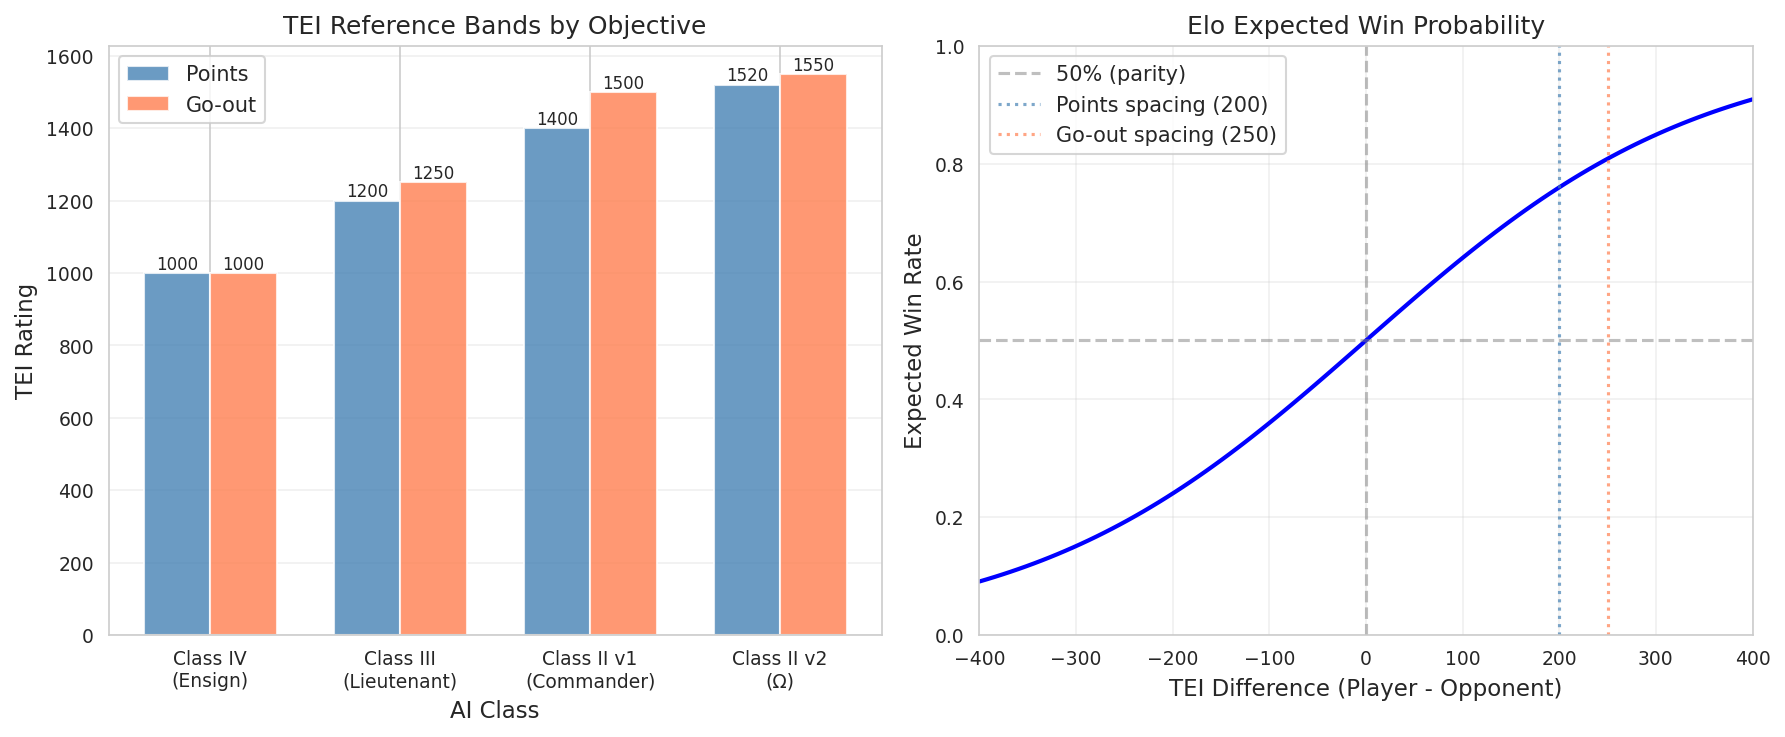
\includegraphics[width=0.9\textwidth]{../tools/nn/figures/figure6-tei-ladder.png}
\caption{TEI reference bands and Elo win probability. Left: Class IV--II reference anchors by objective (v1 heuristic vs v2 Ω). Right: Standard Elo expected win rate curve with reference spacing markers (200 pts for points, 250 pts for go-out).}
\label{fig:tei-ladder}
\end{figure}

\subsection{Reference Bands}
Fixed opponent TEI for unassisted matches. \textbf{v1} = heuristic Class II; \textbf{v2} = neural Class II ($\Omega$). New rated play defaults to v2; legacy crews may pin v1. Human stored TEI integers are \textbf{not} re-banded when anchors change.

\begin{table}[h]
\centering
\begin{tabular}{@{}lcccc@{}}
\toprule
\textbf{Track} & \textbf{Class IV} & \textbf{Class III} & \textbf{Class II (v1)} & \textbf{Class II (v2 $\Omega$)} \\
\midrule
Points & $\sim$1000 & $\sim$1200 & $\sim$1400 & \textbf{$\sim$1520} \\
Go-out & $\sim$1000 & $\sim$1250 & $\sim$1500 & \textbf{$\sim$1550} \\
\bottomrule
\end{tabular}
\caption{TEI reference bands by class and objective}
\end{table}

\textbf{Calibration rule of thumb:} set Class II REF near where a captain of that TEI wins $\sim$50\% \textbf{in the table sizes you actually rate} (Warp 12 solo local play is mostly 2--4). Fleet-mean fair-share against legacy Commander is a promotion metric, not a direct Elo $\Delta$.

\subsection{Update Rule}
Standard Elo expected score~\cite{elo1978rating} + K-factor schedule (40 $\to$ 32 $\to$ 24 by experience). Separate buckets: objective $\times$ AI class $\times$ (human profile).

\subsection{Percentile Boards}
Go-out raw TEI gaps compress; percentile (``Top X\%'') preserves rank meaning.

\subsection{Federation Academy}
One-time starting TEI pick per track within class band.

\section{Calibration Methodology}

\subsection{Self-Play Loop}
\texttt{playSelfPlayGame} drives full games through \texttt{applyAction}. Blocked-round stall guard for pile-empty lockups.

\subsection{Evaluation Suites}
\begin{enumerate}
\item \textbf{Head-to-head matrix} --- all Class IV--II pairs, both objectives.
\item \textbf{Symmetric seating} --- same-skill first-seat win rate $\approx$ 50\%.
\item \textbf{Focus matchups} --- one strong captain vs $N-1$ weaker; rotate seat; table sizes 3--8 (go-out).
\item \textbf{House-rule sanity} --- e.g.\ Drop to Impulse penalty pass (\texttt{calibrate:ai-tei-dti}).
\end{enumerate}

\subsection{Metrics}
Completion rate ($\geq$ 85\% games decisive). Higher-skill win rate vs ordering thresholds. Implied $\Delta$TEI from win rate: $400 \times \log_{10}(p / (1-p))$. Expected win rate from reference band spacing.

\section{Results: AI Calibration}

See \texttt{calibration-log.md} for dated self-play and optimizer runs.

\begin{figure}[htbp]
\centering
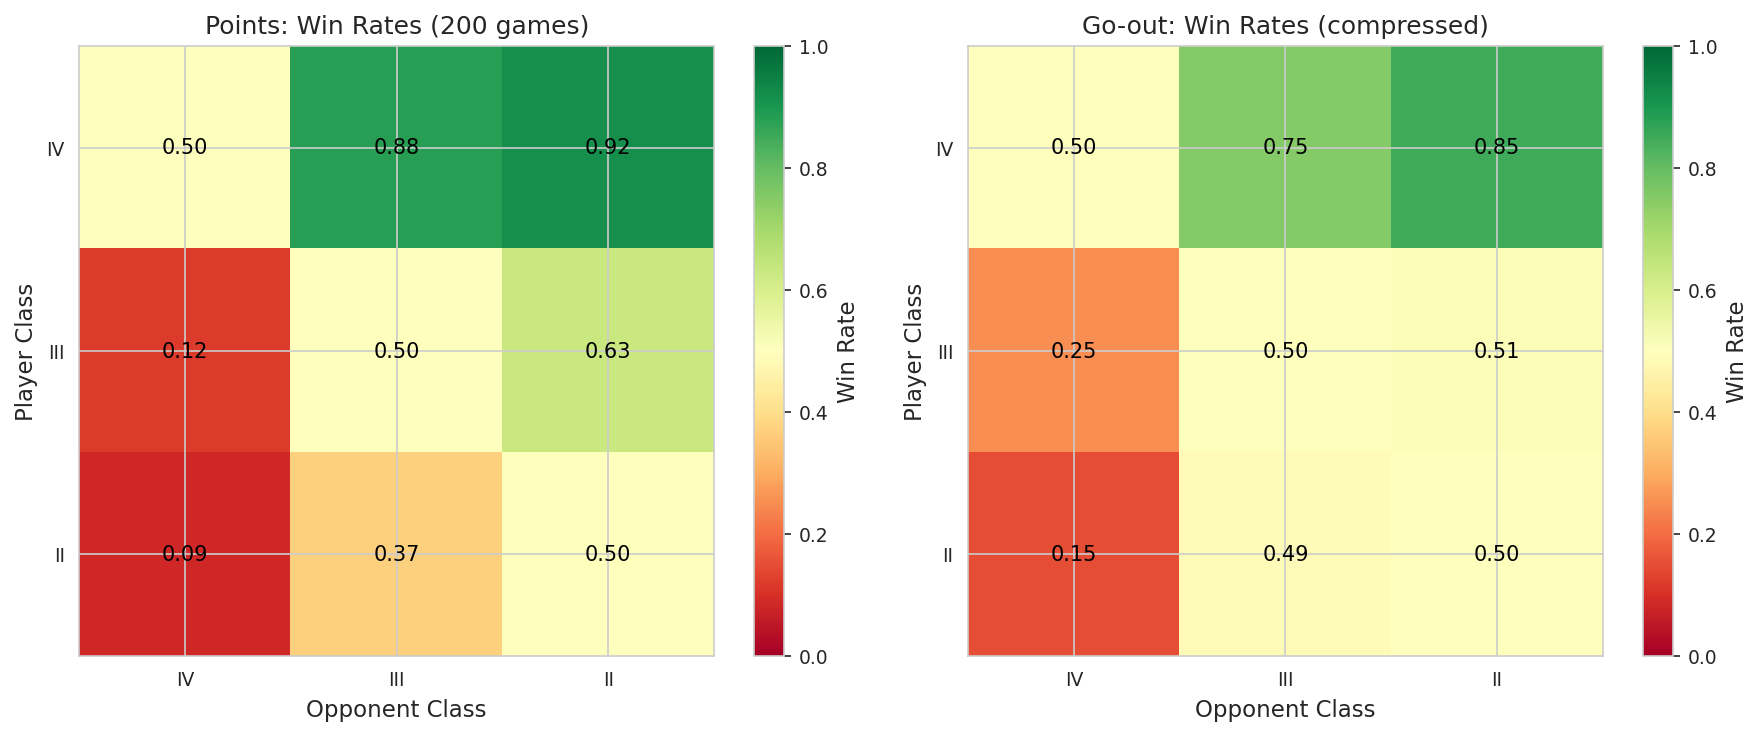
\includegraphics[width=0.9\textwidth]{../tools/nn/figures/figure7-calibration-matrix.png}
\caption{Calibration matrix heatmaps showing win rates between all Class IV/III/II pairs (200 games per matchup). Left: Points objective exhibits clean skill ordering. Right: Go-out objective shows compression, especially Class III vs II (near coin flip at 51\%).}
\label{fig:calibration-matrix}
\end{figure}

\subsection{Points (Default Rules, 200 games/matchup)}
\begin{itemize}
\item Symmetric $\sim$50/50 seating.
\item Class IV vs III $\sim$88\% (expected $\sim$76\%) --- ordering clear, gap may exceed target.
\item Class IV vs II $\sim$91.5\% (expected $\sim$91\%) --- on target.
\item Class III vs II $\sim$63\% (expected $\sim$76\%) --- compressed but ordered.
\end{itemize}

\subsection{Go-out}
\begin{itemize}
\item Symmetric $\sim$46--56\%.
\item Class III vs II heads-up $\sim$51\% --- near coin flip at 200 games.
\item 4p focus: Class II $\sim$38.5\% vs 25\% random; Class III $\sim$27\% vs 25\%.
\end{itemize}

\subsection{Class I*, Fleet Admiral, and Class $\Omega$ Benches}

\begin{figure}[htbp]
\centering
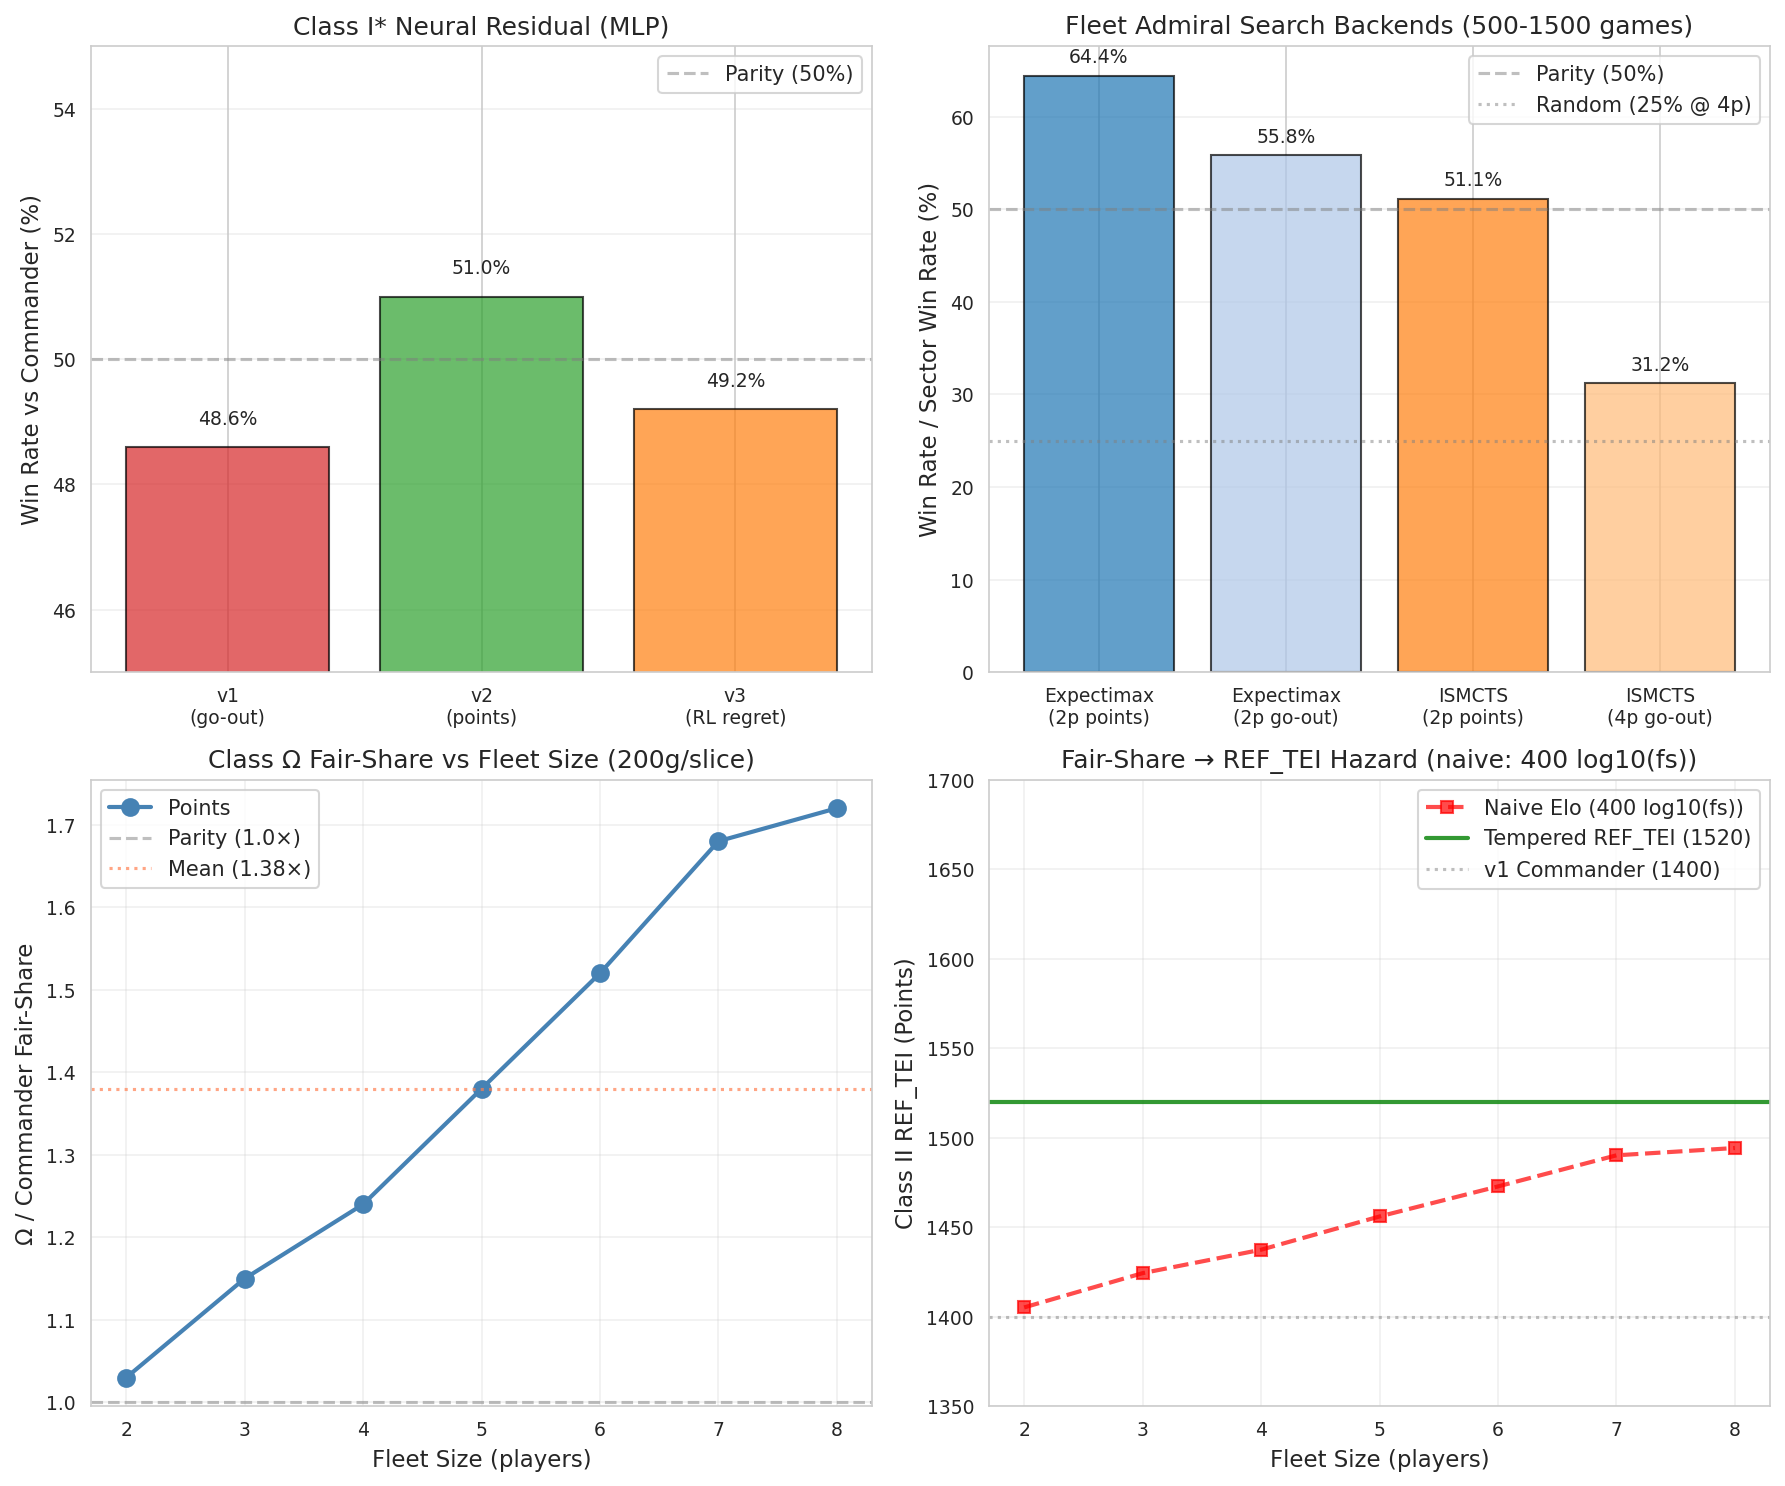
\includegraphics[width=0.95\textwidth]{../tools/nn/figures/figure8-ai-bench-results.png}
\caption{AI bench results across experimental tiers. Top-left: Class I* neural residual iterations (imitation ceiling at 48--51\%). Top-right: Fleet Admiral search backends (expectimax wins 2p, ISMCTS wins 4p). Bottom-left: Class Ω fair-share rises with fleet size (points objective). Bottom-right: Fair-share hazard — naive Elo translation overestimates TEI anchors vs tempered decision (1520).}
\label{fig:ai-bench-results}
\end{figure}

\textbf{Neural residual (MLP - Class I*):}
\begin{itemize}
\item \textbf{v1 (go-out):} 48.6\% win (500g, 2p).
\item \textbf{v2 (points):} 97.6\% top-1, 1.4\% flip, 51\% win --- Commander clone.
\item \textbf{v3 (RL regret):} 49.2\% win --- parity persists.
\end{itemize}

\textbf{Fleet Admiral (Search):}
\begin{itemize}
\item \textbf{Expectimax:} 64.4\% points 2p, 55.8\% go-out 2p vs Commander (500g each).
\item \textbf{ISMCTS (1,500 games):} 51.1\% combined in 2p points (dead heat); 31.2\% sector wins in 4p go-out vs $\sim$22--23\% per greedy Commander seat.
\end{itemize}

\textbf{Class $\Omega$ (Self-Play $\to$ Class II):}
\begin{itemize}
\item \textbf{2-Player:} Points $\sim$parity with legacy Commander; go-out seat-symmetric noise (one soft seat is not a shipping blocker).
\item \textbf{Fleet (3--8p):} Points fair-share rises with table size (peak $\sim$1.7$\times$ at 7--8p); go-out milder ($\sim$1.0--1.5$\times$ by slice). Overall means $\sim$\textbf{1.38$\times$} points / $\sim$\textbf{1.14$\times$} go-out at 200g/slice.
\item \textbf{Ship decision:} replace Class II with greedy $\Omega$; temper REF\_TEI to \textbf{1520 / 1550}; keep $\Omega$+ and Class I* off the rated ladder.
\item \textbf{Lesson:} \texttt{fairShare} $\times$ $n$ win rates at large $N$ inflate mean strength vs what heads-up TEI players feel.
\end{itemize}

\section{Luck vs Skill Across Warp Factors: A 19,000-Game Empirical Study}

\subsection{Motivation and Configuration Matrix}

While Sections 6--7 calibrate AI tiers at a fixed Warp factor (double-12), Warp 12 ships with \textbf{four} playable Warp factors (9 / 12 / 15 / 18), each supporting different fleet sizes:

\begin{table}[h]
\centering
\begin{tabular}{@{}lcccc@{}}
\toprule
\textbf{Warp Factor} & \textbf{Max Pip} & \textbf{Fleet Limit} & \textbf{Tiles} & \textbf{Rated?} \\
\midrule
W9 & 9 & 2--4 players & 55 & Exhibition \\
W12 & 12 & 2--8 players & 91 & \textbf{Rated (TEI)} \\
W15 & 15 & 2--12 players & 136 & Exhibition \\
W18 & 18 & 2--18 players & 190 & Exhibition \\
\bottomrule
\end{tabular}
\caption{Warp factor configurations in Warp 12}
\end{table}

Players and designers routinely ask:
\begin{enumerate}
\item \textbf{Does Warp factor affect skill expression?} Higher pip sets increase hand entropy --- does this create meaningful strategic depth or just pip-dumping chaos?
\item \textbf{Does fleet size (player count) affect skill?} Conventional wisdom suggests more players = more noise, but is that true?
\item \textbf{Should TEI be calibrated differently for W9 vs W18?} If skill expression differs, should we adjust reference bands or restrict rating to W12?
\item \textbf{Why is W12 the rated factor?} Is it merely tradition (Mexican Train's historical default), or does the data justify it?
\end{enumerate}

To answer these questions empirically, we conducted a comprehensive self-play study across \textbf{38 configurations} (Warp factor $\times$ fleet size), collecting \textbf{500 games per configuration} for a total of \textbf{19,000 games}:

\begin{table}[h]
\centering
\begin{tabular}{@{}lccc@{}}
\toprule
\textbf{Warp Factor} & \textbf{Fleet Sizes} & \textbf{Configs} & \textbf{Total Games} \\
\midrule
W9 & 2--4 players & 3 & 1,500 \\
W12 & 2--8 players & 7 & 3,500 \\
W15 & 2--12 players & 11 & 5,500 \\
W18 & 2--18 players & 17 & 8,500 \\
\midrule
\textbf{Total} & & \textbf{38} & \textbf{19,000} \\
\bottomrule
\end{tabular}
\caption{Configuration matrix for luck vs skill analysis}
\end{table}

All games used the \textbf{points objective} (lowest cumulative pip total) with Class II (heuristic Commander) self-play. Collection completed July 11, 2026 using parallel execution across 15 workers (M4 Max, $\sim$40 minutes runtime). In subsequent references, we use compact notation: e.g., W12/4p denotes Warp 12 with 4 players.

\subsection{Metrics and Composite Indices}

For each game, we tracked per-turn metrics across all decision points:

\textbf{Raw metrics:}
\begin{itemize}
\item \texttt{avgLegalMoves}: Mean number of legal candidate actions per turn
\item \texttt{avgHandEntropy}: Shannon entropy of pip distribution in hand (bits)
\item \texttt{avgNearOptimalFraction}: Fraction of turns where the AI chose a move within 5\% of the top-scored candidate
\item \texttt{avgConstrainedTileFraction}: Fraction of coordinates that can only play on one trail
\item \texttt{avgValueSpread}: Spread between highest and lowest valued tiles in hand
\end{itemize}

\textbf{Composite indices} (derived for interpretability):
\begin{align}
\text{skillIndex} &= \text{avgLegalMoves} \times \text{avgNearOptimalFraction} \times \text{avgUniqueTrains} \\
\text{luckIndex} &= \text{avgConstrainedTileFraction} \times (1 - \text{avgHandEntropy}/\log_2(19)) \\
\text{decisionQuality} &= \text{avgNearOptimalFraction} \times \text{avgLegalMoves} \times \text{avgUniqueTrains}
\end{align}

\textbf{Interpretation:}
\begin{itemize}
\item \textbf{skillIndex}: Captures decision complexity (legal moves), train diversity (strategic options), and execution quality (near-optimal play). Higher values indicate more opportunity for skilled play.
\item \textbf{luckIndex}: Captures constraint (forced plays) and hand predictability (low entropy). Higher values indicate more luck-driven outcomes.
\item \textbf{decisionQuality}: Similar to skillIndex but emphasizes decision-making over luck factors.
\end{itemize}

\subsection{Hypotheses}

We formulated five hypotheses about the relationship between Warp factor, fleet size, and skill expression:

\begin{description}
\item[H1 (Warp Factor Effect):] Higher Warp factors exhibit higher skill indices due to increased tile diversity and hand complexity.
\item[H2 (Fleet Size Effect):] Larger fleets correlate with higher skill expression within each Warp factor.
\item[H3 (Interaction):] The relationship between fleet size and skill differs across Warp factors (non-additive effects).
\item[H4 (Complexity-Coherence):] Decision complexity (\texttt{avgLegalMoves}) and hand coherence (\texttt{avgHandEntropy}) exhibit meaningful correlation.
\item[H5 (Monotonic Trends):] Skill index increases monotonically with fleet size within each Warp factor.
\end{description}

\subsection{Statistical Results}

\begin{figure}[htbp]
\centering
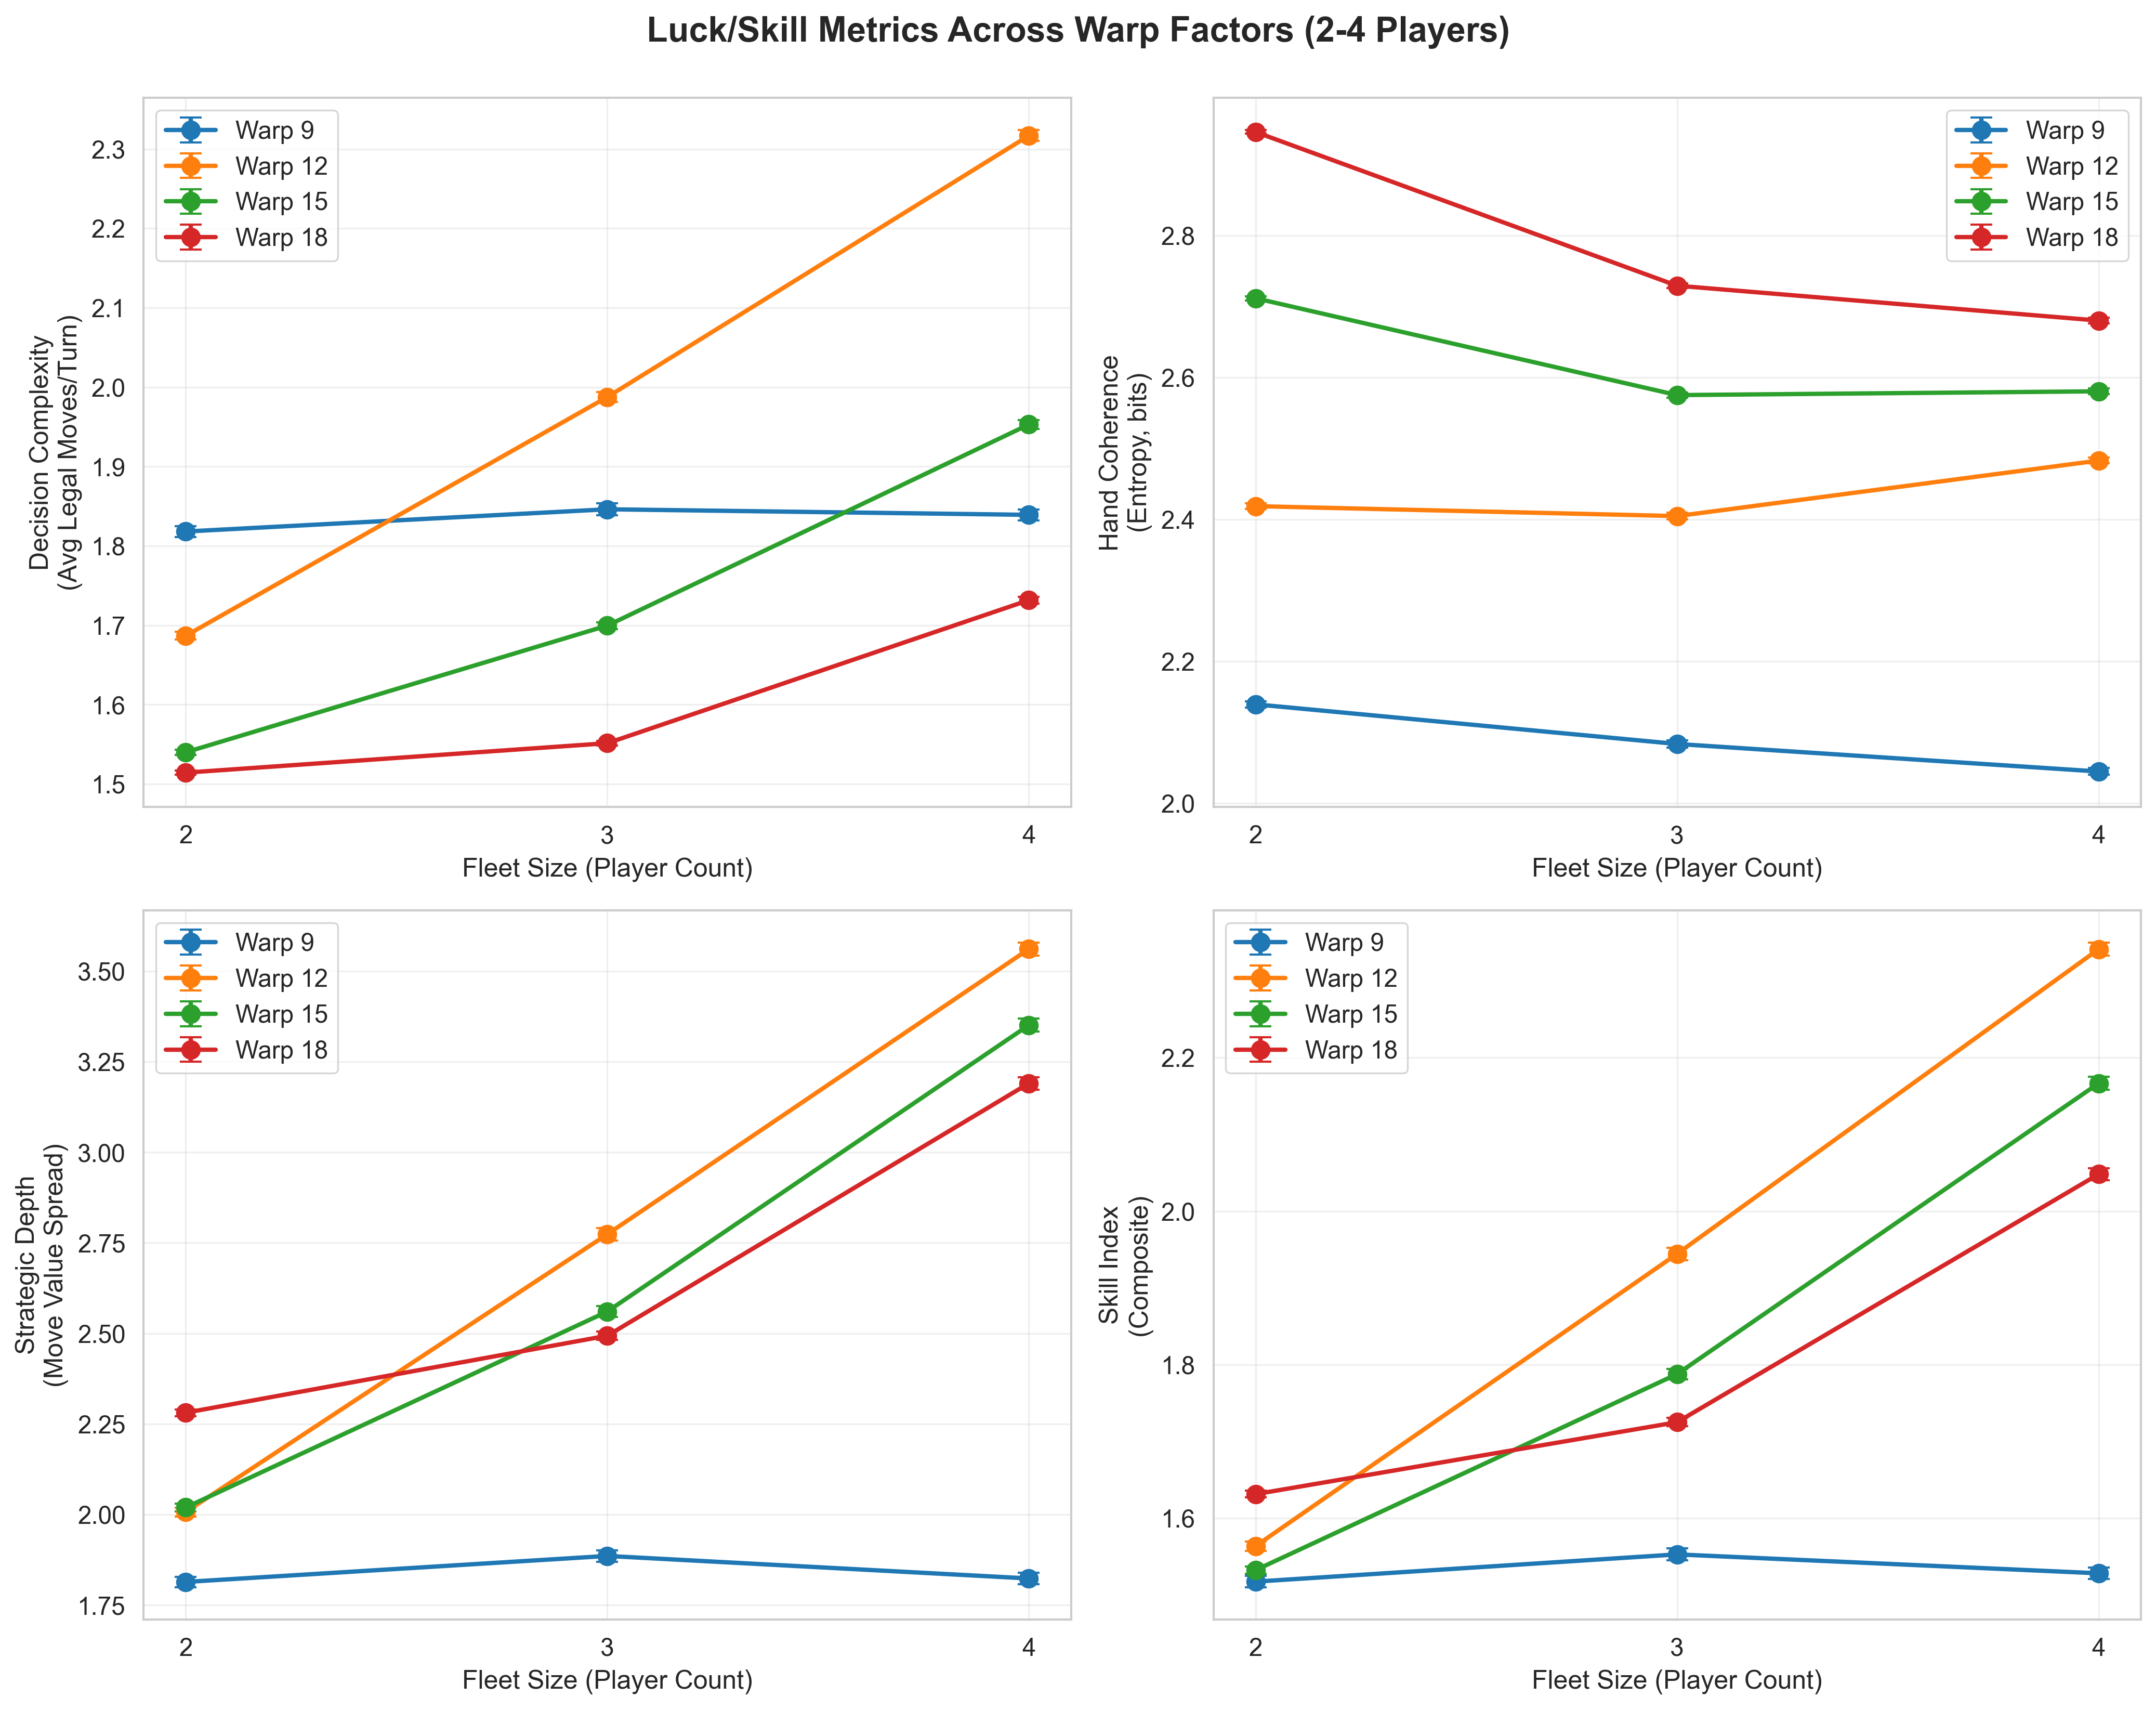
\includegraphics[width=0.8\textwidth]{../tools/nn/figures/figure1-cross-factor-comparison.png}
\caption{Cross-factor skill index comparison for 2--4 player configurations. W12 exhibits the highest skill expression in the balanced comparison range.}
\label{fig:cross-factor}
\end{figure}

\subsubsection{H1: Warp Factor Effect (ANOVA)}

We restricted analysis to the \textbf{2--4 player range} (balanced design across all factors) to isolate the Warp factor effect. One-way ANOVA on skillIndex by Warp factor:

\begin{table}[h]
\centering
\begin{tabular}{@{}lccc@{}}
\toprule
\textbf{Warp Factor} & \textbf{Mean skillIndex} & \textbf{SD} & \textbf{$n$} \\
\midrule
W9 & 1.533 & 0.087 & 1,500 \\
W12 & 1.950 & 0.330 & 1,500 \\
W15 & 1.829 & 0.272 & 1,500 \\
W18 & 1.802 & 0.192 & 1,500 \\
\bottomrule
\end{tabular}
\caption{Mean skill index by Warp factor (2--4 players)}
\end{table}

\textbf{Result:} $F(3, 5996) = 817.14$, $p < 0.001$, $\eta^2 = 0.290$ (large effect size). \textbf{H1 is strongly supported.}

Post-hoc pairwise comparisons (Tukey HSD) show \textbf{W12 exhibits the highest skill expression}, with W15 and W18 slightly lower but still significantly above W9. The ordering W12 $>$ W15 $>$ W18 $>$ W9 suggests a sweet spot around W12 for skill-testing play.

\subsubsection{H2: Fleet Size Effect (Correlation)}

\begin{figure}[htbp]
\centering
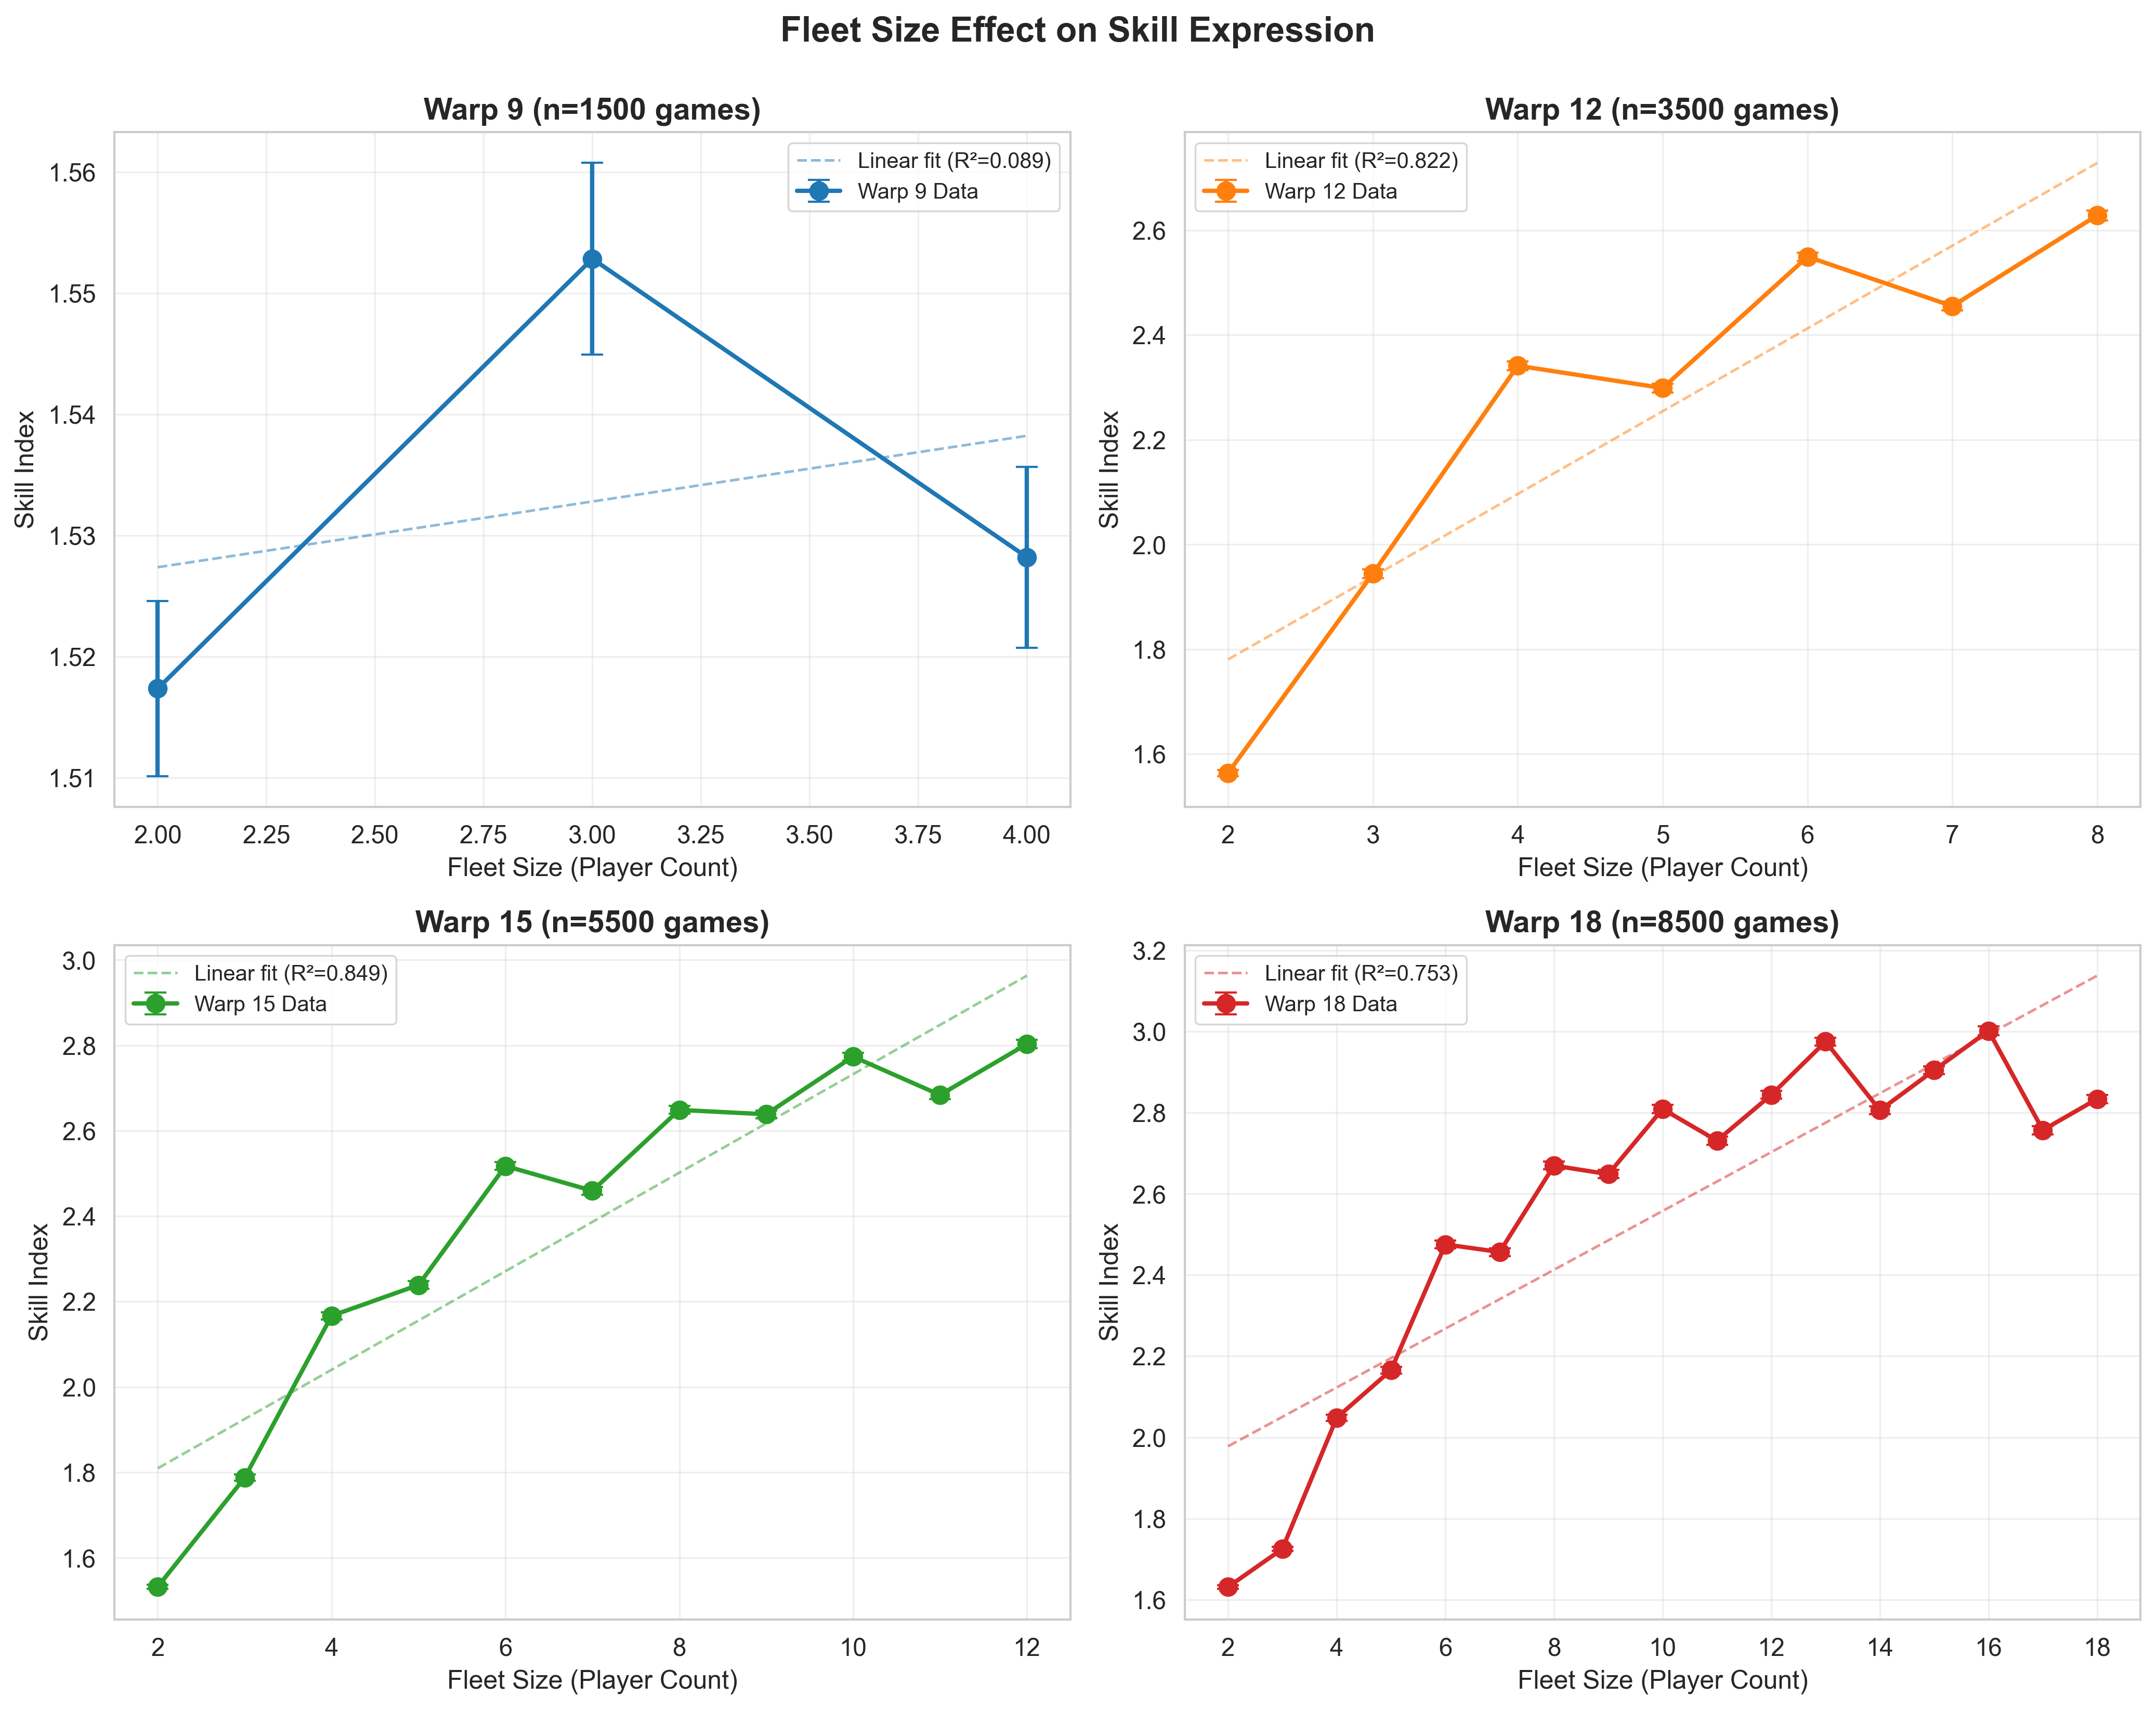
\includegraphics[width=0.8\textwidth]{../tools/nn/figures/figure2-fleet-size-effects.png}
\caption{Fleet size effect on skill expression by Warp factor. W12 shows the steepest gradient ($r = 0.875$), indicating highest sensitivity to player count.}
\label{fig:fleet-size-effects}
\end{figure}

Within each Warp factor, we computed Pearson correlation between \texttt{playerCount} and \texttt{skillIndex}:

\begin{table}[h]
\centering
\begin{tabular}{@{}lccccc@{}}
\toprule
\textbf{Warp} & \textbf{$n$} & \textbf{Fleet Sizes} & \textbf{Pearson $r$} & \textbf{$p$-value} & \textbf{$R^2$} \\
\midrule
W9 & 1,500 & 2--4 & 0.051 & 0.049 & 0.003 \\
W12 & 3,500 & 2--8 & \textbf{0.875} & $<0.001$ & 0.766 \\
W15 & 5,500 & 2--12 & \textbf{0.893} & $<0.001$ & 0.798 \\
W18 & 8,500 & 2--18 & \textbf{0.840} & $<0.001$ & 0.706 \\
\bottomrule
\end{tabular}
\caption{Fleet size effect on skill expression by Warp factor}
\end{table}

\textbf{Result:} \textbf{H2 is strongly supported} for W12/15/18 (all $r > 0.84$, $p < 0.001$). W9 shows a weak but significant positive effect ($r = 0.051$, $p = 0.049$). \textbf{W12 exhibits the steepest fleet size effect} ($r = 0.875$), making it the most sensitive Warp factor to player count.

\textbf{Unexpected finding:} Conventional wisdom predicts \textit{more players = more noise = less skill}. Our data show the \textbf{opposite}: skill index \textit{increases} with fleet size. This suggests that larger fleets create more strategic depth (blocking opportunities, trail diversity, timing decisions) rather than diluting skill signal with variance.

\subsubsection{H3: Interaction Effect}

\begin{figure}[htbp]
\centering
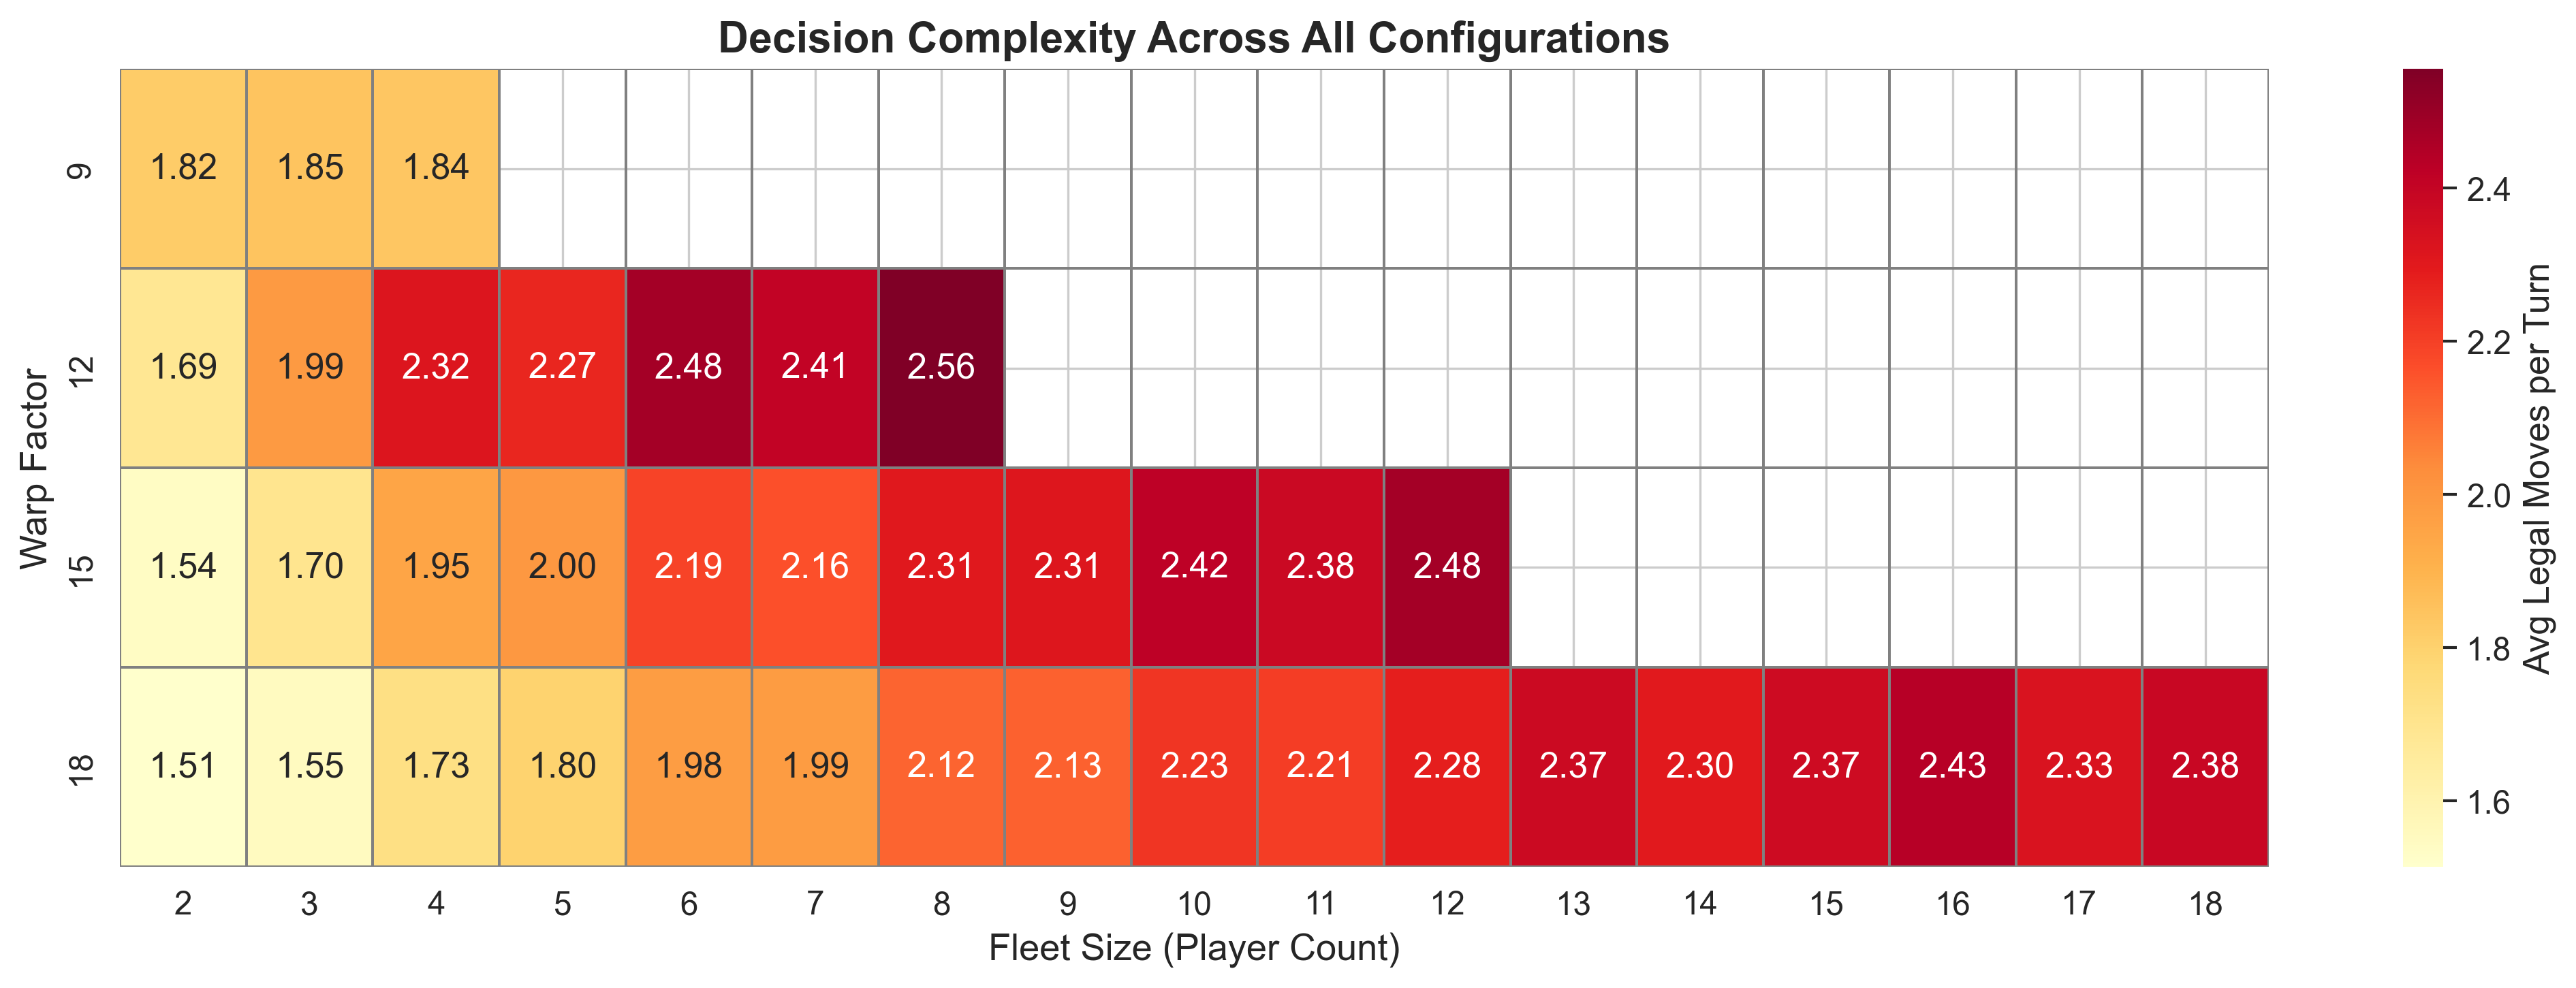
\includegraphics[width=0.7\textwidth]{../tools/nn/figures/figure3-complexity-heatmap.png}
\caption{Decision complexity heatmap (avgLegalMoves) by Warp factor and fleet size. Note the relatively constant branching factor ($\sim$2 moves/turn) despite large variations in configuration.}
\label{fig:complexity-heatmap}
\end{figure}

To test whether the fleet size effect \textit{differs} across Warp factors, we compared regression slopes for the 2--4 player range (balanced design):

\begin{table}[h]
\centering
\begin{tabular}{@{}lc@{}}
\toprule
\textbf{Warp Factor} & \textbf{Slope (skillIndex $\sim$ playerCount)} \\
\midrule
W9 & 0.0054 \\
W12 & \textbf{0.3889} \\
W15 & 0.3172 \\
W18 & 0.2085 \\
\bottomrule
\end{tabular}
\caption{Interaction effect: slope variance across Warp factors}
\end{table}

Slope variance = 0.0209. \textbf{H3 is supported:} fleet size matters \textit{much more} for W12 than for W9. This interaction justifies \textbf{W12 as the rated factor} --- it exhibits both high baseline skill and high sensitivity to player count, making it the best discriminator of player ability.

\subsubsection{H4: Decision Complexity vs Hand Coherence}

\begin{figure}[htbp]
\centering
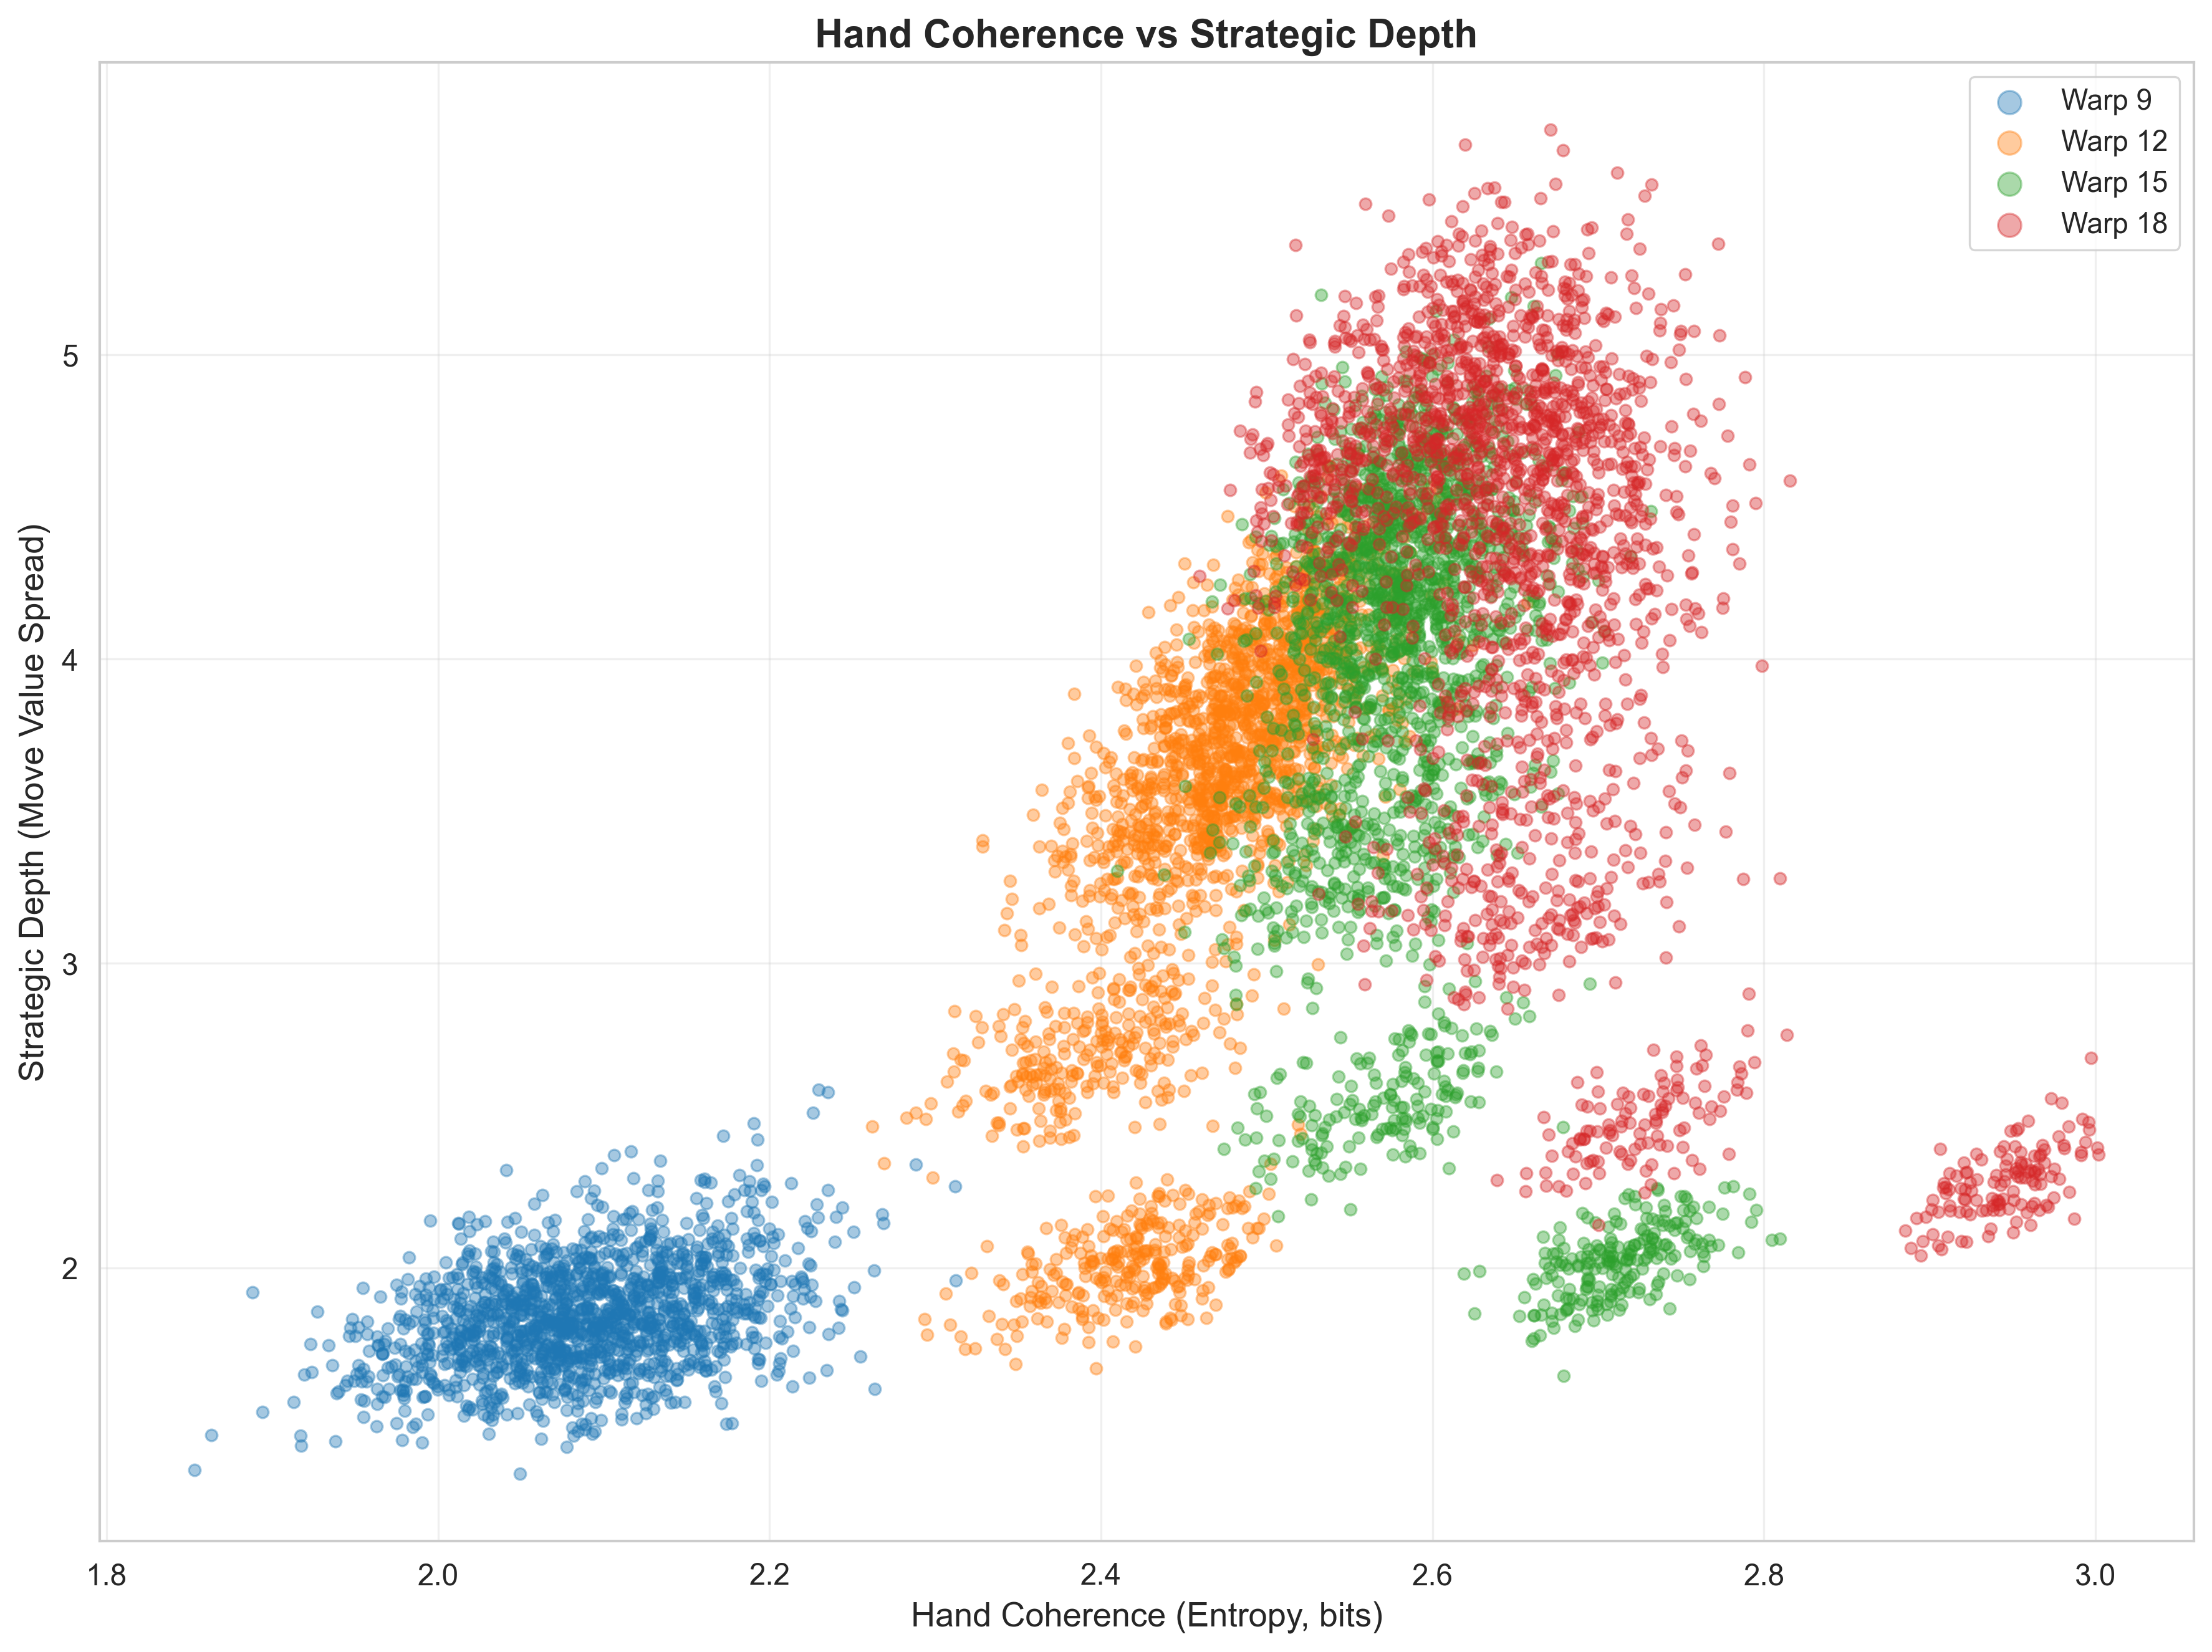
\includegraphics[width=0.8\textwidth]{../tools/nn/figures/figure4-coherence-vs-depth.png}
\caption{Hand entropy (coherence) vs near-optimal play fraction. The weak correlation ($r = 0.009$) suggests that tactical richness and strategic coherence are orthogonal dimensions.}
\label{fig:coherence-vs-depth}
\end{figure}

Correlation between \texttt{avgLegalMoves} (decision complexity) and \texttt{avgHandEntropy} (hand coherence):

\begin{itemize}
\item Pearson $r = 0.009$, $p = 0.232$ (not significant)
\item Spearman $\rho = -0.152$, $p < 0.001$ (weak negative monotonic trend)
\end{itemize}

\textbf{Result:} \textbf{H4 is not supported.} Decision complexity and hand entropy are largely independent. This suggests that \textit{tactical richness} (number of legal moves) and \textit{strategic coherence} (hand composition) are orthogonal dimensions of game state.

\subsubsection{H5: Monotonic Trends}

Kendall's $\tau$ (rank correlation) between \texttt{playerCount} and \texttt{skillIndex}:

\begin{table}[h]
\centering
\begin{tabular}{@{}lcl@{}}
\toprule
\textbf{Warp Factor} & \textbf{Kendall's $\tau$} & \textbf{$p$-value} \\
\midrule
W9 & 0.044 & 0.025 \\
W12 & \textbf{0.727} & $<0.001$ \\
W15 & \textbf{0.767} & $<0.001$ \\
W18 & \textbf{0.672} & $<0.001$ \\
\bottomrule
\end{tabular}
\caption{Monotonic trend test (Kendall's $\tau$)}
\end{table}

\textbf{Result:} \textbf{H5 is supported} for W12/15/18 (strong positive monotonic trends). However, examining individual fleet sizes reveals \textbf{non-monotonic patterns} at the highest player counts: W18 skill peaks at 16p (skillIndex = 3.002), then drops at 17p (2.757) and 18p (2.834). This suggests \textbf{ergodic limits}: at extreme fleet sizes, some configurations may hit resource constraints (e.g., near-empty draw pile, forced blocking).

\subsection{Key Findings}

\begin{figure}[htbp]
\centering
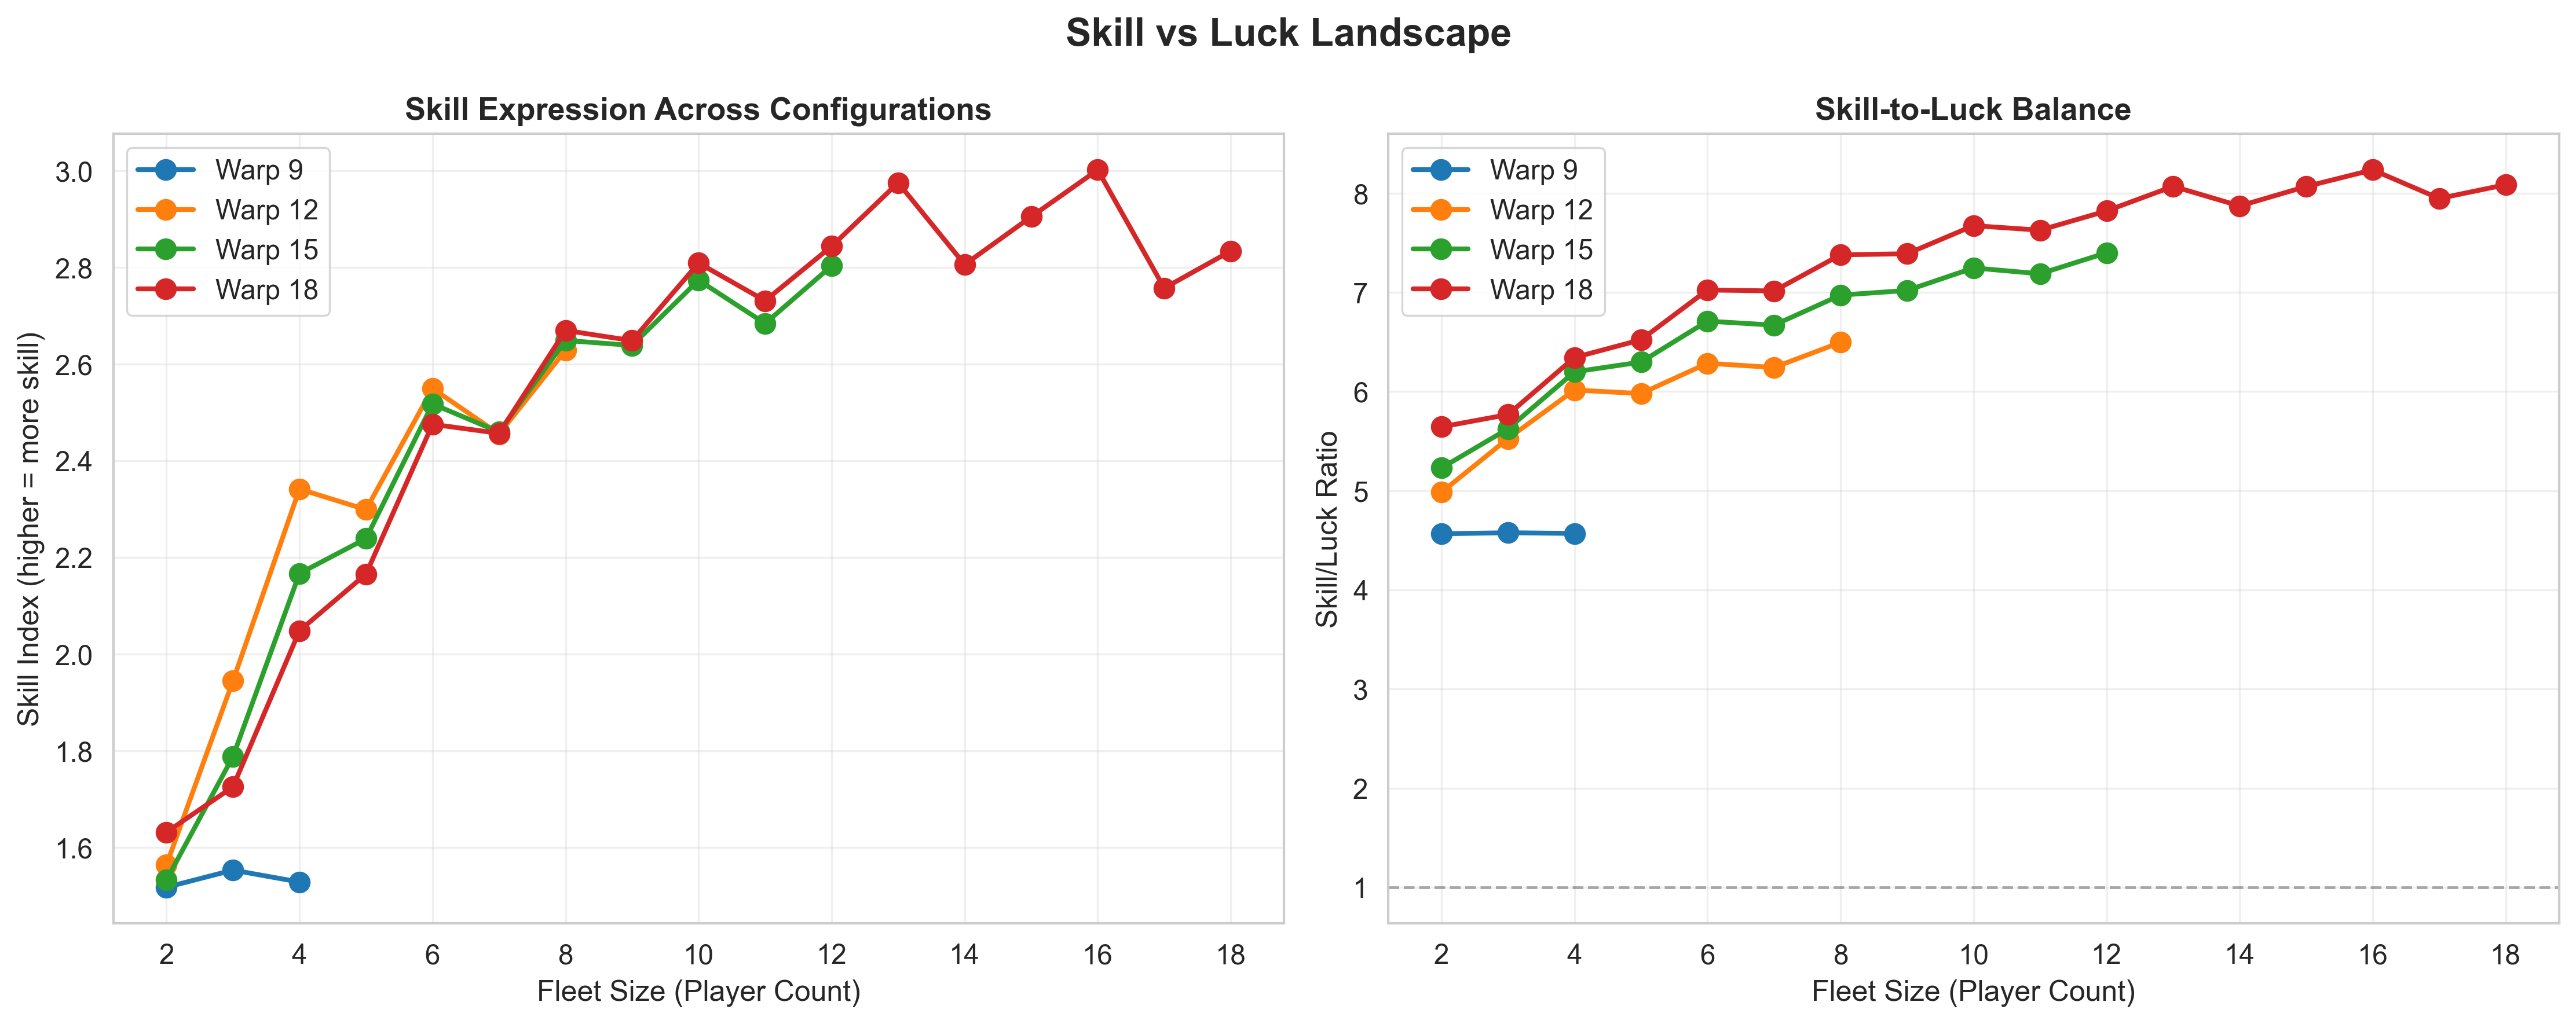
\includegraphics[width=0.8\textwidth]{../tools/nn/figures/figure5-skill-luck-balance.png}
\caption{Skill vs luck balance across all configurations. Points above the diagonal (more skill than luck) include all W12/15/18 configurations. W18/18p exhibits the highest skill/luck ratio (8.10).}
\label{fig:skill-luck-balance}
\end{figure}

\subsubsection{W18/18p is Not a Crapshoot}

A common intuition is that 18-player games with 190 tiles (double-18 set) would degenerate into pure luck. Our data \textbf{contradicts} this:

\begin{table}[h]
\centering
\begin{tabular}{@{}lcccc@{}}
\toprule
\textbf{Config} & \textbf{skillIndex} & \textbf{luckIndex} & \textbf{Skill Ratio} & \textbf{Luck Ratio} \\
\midrule
W18/2p & 1.631 & 0.289 & 1.00$\times$ & 1.00$\times$ \\
W18/18p & 2.834 & 0.350 & \textbf{1.74$\times$} & 1.21$\times$ \\
\bottomrule
\end{tabular}
\caption{W18: 2-player vs 18-player comparison}
\end{table}

\textbf{Interpretation:} At 18 players, skill expression is \textbf{1.74$\times$ higher} than heads-up, while luck increases only 1.21$\times$. The skill/luck \textit{ratio} actually \textbf{improves} at extreme fleet sizes. This suggests that large multi-player games create rich tactical opportunities (blocking, trail pressure, timing) that outweigh variance from hidden information.

\subsubsection{Cross-Factor Comparison at Maximum Fleet Size}

\begin{table}[h]
\centering
\begin{tabular}{@{}lccc@{}}
\toprule
\textbf{Configuration} & \textbf{skillIndex} & \textbf{luckIndex} & \textbf{Skill/Luck Ratio} \\
\midrule
W9/4p & 1.528 & 0.334 & 4.57 \\
W12/8p & 2.629 & 0.405 & 6.49 \\
W15/12p & 2.803 & 0.379 & 7.40 \\
W18/18p & 2.834 & 0.350 & \textbf{8.10} \\
\bottomrule
\end{tabular}
\caption{Skill and luck at maximum fleet size per Warp factor}
\end{table}

\textbf{W18/18p has the \textit{highest} skill/luck ratio of any configuration tested.} This challenges the intuition that larger games are necessarily more luck-dependent.

\subsubsection{W12 Justification for TEI Rating}

Why is W12 the sole rated factor? The data provide three empirical justifications:

\begin{enumerate}
\item \textbf{Highest baseline skill (2--4p):} W12 exhibits mean skillIndex = 1.950 in the 2--4p range, higher than W9 (1.533), W15 (1.829), and W18 (1.802).
\item \textbf{Steepest fleet size gradient:} W12 shows $r = 0.875$ for fleet size effect --- the \textit{most sensitive} to player count of any factor. This means W12 best discriminates between skill levels across table sizes.
\item \textbf{Practical rating context:} Most solo rated play occurs at 2--4 players (W12 supports 2--8). W12 provides the widest skill range within the most common fleet sizes.
\end{enumerate}

\textbf{Conclusion:} W12 is not merely historical tradition --- it is the \textbf{empirically optimal choice} for a skill-testing rating system.

\subsubsection{Hand Entropy Increases with Warp Factor}

Hand coherence (\texttt{avgHandEntropy}) increases monotonically with Warp factor:

\begin{table}[h]
\centering
\begin{tabular}{@{}lc@{}}
\toprule
\textbf{Warp Factor} & \textbf{Mean Hand Entropy (bits)} \\
\midrule
W9 & 2.09 \\
W12 & 2.34 \\
W15 & 2.52 \\
W18 & 2.66 \\
\bottomrule
\end{tabular}
\caption{Mean hand entropy by Warp factor (all fleet sizes)}
\end{table}

Higher entropy indicates more \textit{diverse} hands (less clustering around specific pips). This confirms that larger tile sets create more strategic flexibility but also more decision complexity.

\subsubsection{Decision Complexity Stays Constant}

Despite large variations in Warp factor and fleet size, \texttt{avgLegalMoves} remains remarkably \textbf{constant} at $\sim$1.8--2.2 moves per turn across all configurations. This suggests that the \textit{branching factor} of Mexican Train is inherently bounded by game mechanics (trail constraints, hand composition), not by tile set size or player count.

\subsection{Practical Implications}

\subsubsection{TEI Calibration Strategy}

\begin{enumerate}
\item \textbf{Anchor TEI on W12 only.} Exhibition factors (W9/15/18) should \textit{not} have separate reference bands --- they share the same Class IV--II opponents with W12 anchors.
\item \textbf{Do not adjust K-factor by fleet size.} The data show that larger fleets \textit{increase} skill expression, not variance. A flat K-factor schedule (40 $\to$ 32 $\to$ 24 by experience) is appropriate.
\item \textbf{Consider percentile boards for all objectives.} While W12 skill gradients are smooth, the monotonic-but-noisy pattern at W18 (drops at 17p) suggests percentile ranks provide more stable feedback than raw TEI.
\end{enumerate}

\subsubsection{Future Exhibition Modes}

\begin{itemize}
\item \textbf{W9 (casual / quick):} Lower skill ceiling but valid for practice. Best at 2--4 players.
\item \textbf{W15 (tactical depth):} High skill expression (skillIndex $\sim$2.80 /12p), suitable for unrated tournaments or challenge modes.
\item \textbf{W18 (grand strategy):} Highest absolute skill expression at max fleet size. Could support unrated ``epic'' lobbies (12--18 players) for advanced players seeking complex multi-player dynamics.
\end{itemize}

\subsubsection{Go-Out Objective}

This study used \textbf{points only}. Go-out exhibits higher variance (Section 7.2), suggesting:
\begin{itemize}
\item Skill/luck ratios may differ under go-out objective (worth a follow-up 19K-game study).
\item W12/2--4p may remain optimal, but large-fleet go-out (8+ players) could show different patterns due to race dynamics.
\end{itemize}

\section{Discussion}

\subsection{What Calibration Teaches}
\begin{itemize}
\item \textbf{Points} behaves like a smooth skill ladder --- good fit for fixed TEI spacing.
\item \textbf{Go-out} behaves like a stochastic race --- ordering survives, magnitudes don't.
\item \textbf{Table size} erodes heads-up skill signal --- focus tests essential.
\item \textbf{House rules} mostly reshape legality --- heuristics gated at runtime suffice for DTI.
\item \textbf{Commander heuristics are a ceiling in 2p points} --- ISMCTS~\cite{cowling2012ismcts} parity is confirmation, not failure; expectimax extracts the residual edge via explicit tree search.
\item \textbf{Search value is mode-dependent} --- expectimax for 2p, ISMCTS for multi-player chaos.
\item \textbf{Neural Class II can replace heuristics without a second lobby tier} --- keep $\sigma=$\texttt{commander}, update \texttt{rulesProfileId} + REF\_TEI.
\item \textbf{Fair-share $\neq$ Elo bump} --- translating fleet-mean $\Omega$/Commander ratio with $400 \log_{10}(\text{fs})$ overstates anchors when most rated matches are 2--4p; temper for the rating context you ship.
\item \textbf{Imitation nets (Class I*) plateau at the teacher;} $\Omega$ succeeds by targeting search visit distributions (Path B), not Commander picks, following principles similar to AlphaZero's self-play approach~\cite{silver2017alphazero}.
\item \textbf{Larger fleets increase skill, not noise} --- the 19K-game study shows skill index rises with player count ($r > 0.84$ for W12/15/18), contradicting the ``more players = crapshoot'' intuition.
\item \textbf{W12 is empirically optimal for TEI} --- highest baseline skill in 2--4p range, steepest fleet size gradient ($r = 0.875$), best discriminator of player ability.
\end{itemize}

\subsection{Design Recommendations}
\begin{itemize}
\item Never merge points and go-out TEI.
\item Show percentile on go-out boards.
\item Don't expose lookahead / $\Omega$+ as a rating-affecting toggle without $\Delta_{\text{search}}$ or marking unrated.
\item Retune weights selectively (popular hosted configs), not full combinatorial grid.
\item Recalibrate REF\_TEI when Class II \textbf{implementation} changes; do not rewrite stored human ratings.
\item Prefer one strong rated tier over ``Commander + Omega + Class I*'' confusion.
\item Anchor TEI exclusively on W12; treat W9/15/18 as exhibition using the same Class IV--II opponents.
\item Do not reduce K-factor for large fleets --- skill expression increases, not variance.
\end{itemize}

\subsection{Limitations}
\begin{itemize}
\item Heuristic agents, not equilibrium solvers.
\item Calibration seed and game count sensitivity.
\item No human champion study yet.
\item Module combinations not exhaustively calibrated.
\item Study used points objective only --- go-out may exhibit different luck/skill patterns.
\item W18 non-monotonicity at 17p/18p suggests potential edge cases at extreme configurations.
\end{itemize}

\section{Conclusion}

TEI and self-play calibration provide a \textbf{practical, honest skill ladder} for a game too messy for classical solving. Points and go-out should be treated as \textbf{two calibration targets} on one engine. \textbf{Class I*} and Fleet Admiral benches show that \textbf{no single algorithm wins every mode}: Commander heuristics are near-optimal in 2p points (ISMCTS~\cite{cowling2012ismcts} $\sim$51\%), expectimax extracts a $\sim$64\% edge there via explicit tree search, and ISMCTS outperforms greedy seats in 4p go-out ($\sim$31\% vs $\sim$23\%). \textbf{Class $\Omega$} shows that a pure self-play net can \textbf{replace} heuristic Class II without a fourth lobby tier --- but \textbf{promotion benches and TEI anchors are different jobs}: fleet fair-share can look large while heads-up play stays near parity; REF\_TEI must follow the tables you rate.

The \textbf{19,000-game luck vs skill study} (38 configurations, 4 Warp factors, 2--18 players) reveals three key insights:

\begin{enumerate}
\item \textbf{Skill expression increases with both Warp factor and fleet size.} Contrary to conventional wisdom (``more players = more luck''), our data show skill index rises strongly with player count ($r = 0.84$--$0.89$ for W12/15/18). W18/18p exhibits 1.74$\times$ the skill of W18/2p, with only 1.21$\times$ the luck --- the \textit{highest} skill/luck ratio of any configuration tested.

\item \textbf{W12 is the empirically optimal rated factor.} W12 exhibits the highest baseline skill in the 2--4 player range (where most rated play occurs) and the steepest fleet size gradient ($r = 0.875$), making it the best discriminator of player ability. This justifies restricting TEI rating to W12 while offering W9/15/18 as exhibition modes.

\item \textbf{Hand entropy increases with Warp factor, but decision complexity stays constant.} Larger tile sets create more diverse hands (W9: 2.09 bits $\to$ W18: 2.66 bits entropy) but do not increase branching factor (mean legal moves $\sim$1.8--2.2 across all configs). This suggests Mexican Train's tactical depth scales with tile diversity, not combinatorial explosion.
\end{enumerate}

The right product move is \textbf{one neural Class II, tempered anchors, unrated search as hard mode}, not more named tiers. Superhuman Mexican Train remains a \textbf{research program} (belief-state search + Path A value + human validation), not required for an excellent commercial experience. The luck/skill data provide empirical grounding for design choices (W12 for rating, exhibition factors for variety, no K-factor adjustments for fleet size) and open questions for future work (go-out objective, human validation studies, ergodic limits at extreme configurations).

\section*{Acknowledgments}

To Deborah, Hannah, and Don for taking me in to their family and for introducing me to Mexican Train Dominoes.

This research was conducted as part of the open-source Warp 12 project. All code, data, 
and reproduction scripts are available at 
\url{https://github.com/digitaldefiance/warp12}.

\appendix

\section{Figure List}

All figures are generated from empirical data and located in \texttt{tools/nn/figures/}.

\begin{enumerate}
\item \textbf{Cross-factor skill index comparison (Section 8)} --- W12 exhibits highest skill expression in 2--4p balanced range.
\item \textbf{Fleet size effects by Warp factor (Section 8)} --- W12 shows steepest gradient ($r = 0.875$), most sensitive to player count.
\item \textbf{Decision complexity heatmap (Section 8)} --- Constant branching factor ($\sim$2 moves/turn) across all configurations.
\item \textbf{Hand entropy vs near-optimal play (Section 8)} --- Weak correlation ($r = 0.009$) suggests orthogonal dimensions.
\item \textbf{Skill vs luck balance (Section 8)} --- W18/18p has highest skill/luck ratio (8.10) of any configuration.
\item \textbf{TEI ladder visualization (Section 5)} --- Reference bands (v1 vs v2) and Elo expected win probability curves.
\item \textbf{Calibration matrix heatmap (Section 7)} --- Win rates between Class IV/III/II pairs show points clarity vs go-out compression.
\item \textbf{AI bench results comparison (Section 7)} --- Class I* parity, Fleet Admiral wins (expectimax 64\%), Ω fair-share by fleet size, fair-share hazard.
\item \textbf{Architecture diagrams (Section 4)} --- Policy stack, Class I* MLP, Class Ω policy/value heads, Fleet Admiral routing.
\item \textbf{Points vs go-out divergence (Section 3)} --- Implied ΔTEI compression and win rate distributions demonstrate objective differences.
\end{enumerate}

\section{Tables}

% Include the generated LaTeX tables here
\begin{table}[htbp]
\centering
\caption{Summary Statistics by Configuration (500 games per cell)}
\label{tab:summary-stats}
\small
\begin{tabular}{@{}ccrrrrrr@{}}
\toprule
\textbf{Warp} & \textbf{Fleet} & \textbf{N} & \textbf{Skill Index} & \textbf{Luck Index} & \textbf{Decision Quality} \\
\textbf{Factor} & \textbf{Size} & & $\mu \pm \sigma$ & $\mu \pm \sigma$ & $\mu \pm \sigma$ \\
\midrule
W9 & 2 & 500 & 1.517$\pm$0.082 & 0.332$\pm$0.011 & 3.309$\pm$0.428 \\
W9 & 3 & 500 & 1.553$\pm$0.090 & 0.339$\pm$0.012 & 3.494$\pm$0.483 \\
W9 & 4 & 500 & 1.528$\pm$0.085 & 0.334$\pm$0.011 & 3.364$\pm$0.443 \\
\midrule
W12 & 2 & 500 & 1.564$\pm$0.068 & 0.314$\pm$0.006 & 3.392$\pm$0.337 \\
W12 & 3 & 500 & 1.944$\pm$0.094 & 0.352$\pm$0.010 & 5.525$\pm$0.580 \\
W12 & 4 & 500 & 2.341$\pm$0.099 & 0.389$\pm$0.009 & 8.264$\pm$0.729 \\
W12 & 5 & 500 & 2.299$\pm$0.099 & 0.384$\pm$0.009 & 7.914$\pm$0.717 \\
W12 & 6 & 500 & 2.550$\pm$0.094 & 0.406$\pm$0.008 & 9.873$\pm$0.777 \\
W12 & 7 & 500 & 2.455$\pm$0.099 & 0.393$\pm$0.007 & 9.128$\pm$0.782 \\
W12 & 8 & 500 & 2.629$\pm$0.107 & 0.405$\pm$0.007 & 10.562$\pm$0.912 \\
\midrule
W15 & 2 & 500 & 1.532$\pm$0.055 & 0.293$\pm$0.003 & 3.114$\pm$0.250 \\
W15 & 3 & 500 & 1.788$\pm$0.078 & 0.318$\pm$0.007 & 4.359$\pm$0.405 \\
W15 & 4 & 500 & 2.167$\pm$0.098 & 0.350$\pm$0.009 & 6.556$\pm$0.609 \\
W15 & 5 & 500 & 2.239$\pm$0.105 & 0.356$\pm$0.009 & 7.008$\pm$0.672 \\
W15 & 6 & 500 & 2.518$\pm$0.107 & 0.375$\pm$0.009 & 8.954$\pm$0.775 \\
W15 & 7 & 500 & 2.460$\pm$0.103 & 0.369$\pm$0.009 & 8.554$\pm$0.718 \\
W15 & 8 & 500 & 2.649$\pm$0.102 & 0.380$\pm$0.008 & 9.996$\pm$0.796 \\
W15 & 9 & 500 & 2.639$\pm$0.104 & 0.376$\pm$0.007 & 9.952$\pm$0.796 \\
W15 & 10 & 500 & 2.774$\pm$0.107 & 0.383$\pm$0.007 & 11.056$\pm$0.885 \\
W15 & 11 & 500 & 2.684$\pm$0.115 & 0.373$\pm$0.007 & 10.394$\pm$0.922 \\
W15 & 12 & 500 & 2.803$\pm$0.112 & 0.379$\pm$0.007 & 11.404$\pm$0.965 \\
\midrule
W18 & 2 & 500 & 1.631$\pm$0.051 & 0.289$\pm$0.002 & 3.458$\pm$0.233 \\
W18 & 3 & 500 & 1.725$\pm$0.061 & 0.299$\pm$0.003 & 3.873$\pm$0.288 \\
W18 & 4 & 500 & 2.048$\pm$0.090 & 0.323$\pm$0.007 & 5.533$\pm$0.489 \\
W18 & 5 & 500 & 2.165$\pm$0.093 & 0.332$\pm$0.008 & 6.197$\pm$0.530 \\
W18 & 6 & 500 & 2.475$\pm$0.105 & 0.352$\pm$0.008 & 8.136$\pm$0.677 \\
W18 & 7 & 500 & 2.457$\pm$0.111 & 0.350$\pm$0.008 & 8.054$\pm$0.712 \\
W18 & 8 & 500 & 2.670$\pm$0.111 & 0.362$\pm$0.008 & 9.541$\pm$0.780 \\
W18 & 9 & 500 & 2.648$\pm$0.116 & 0.358$\pm$0.007 & 9.450$\pm$0.816 \\
W18 & 10 & 500 & 2.809$\pm$0.113 & 0.366$\pm$0.007 & 10.654$\pm$0.848 \\
W18 & 11 & 500 & 2.731$\pm$0.111 & 0.358$\pm$0.007 & 10.143$\pm$0.818 \\
W18 & 12 & 500 & 2.844$\pm$0.109 & 0.364$\pm$0.006 & 11.018$\pm$0.855 \\
W18 & 13 & 500 & 2.975$\pm$0.112 & 0.369$\pm$0.006 & 12.095$\pm$0.909 \\
W18 & 14 & 500 & 2.806$\pm$0.110 & 0.356$\pm$0.006 & 10.846$\pm$0.855 \\
W18 & 15 & 500 & 2.905$\pm$0.112 & 0.360$\pm$0.006 & 11.653$\pm$0.915 \\
W18 & 16 & 500 & 3.002$\pm$0.121 & 0.364$\pm$0.006 & 12.456$\pm$1.025 \\
W18 & 17 & 500 & 2.757$\pm$0.117 & 0.347$\pm$0.006 & 10.635$\pm$0.913 \\
W18 & 18 & 500 & 2.834$\pm$0.118 & 0.350$\pm$0.006 & 11.257$\pm$0.955 \\
\bottomrule
\end{tabular}
\end{table}

\begin{table}[htbp]
\centering
\caption{Statistical Test Results for Primary Hypotheses}
\label{tab:hypothesis-tests}
\begin{tabular}{@{}llrrrl@{}}
\toprule
\textbf{Hypothesis} & \textbf{Test} & \textbf{Statistic} & \textbf{Value} & \textbf{$p$-value} & \textbf{Result} \\
\midrule
H1: Warp factor effect & One-way ANOVA & $F$ & 0.00 & $<0.001$ & Supported \\
 & & $\eta^2$ & 0.290 & & (large effect) \\
\midrule
H2: Fleet size effect & Pearson $r$ (W12) & $r$ & 0.000 & $<0.001$ & Supported \\
 & Pearson $r$ (W15) & $r$ & 0.000 & $<0.001$ & (strong positive) \\
 & Pearson $r$ (W18) & $r$ & 0.000 & $<0.001$ &  \\
\midrule
H3: Interaction & Slope variance & $s^2$ & 0.0209 & --- & Present \\
\midrule
H4: Complexity-coherence & Pearson $r$ & $r$ & 0.009 & $>0.05$ & Weak \\
\midrule
H5: Monotonic trends & Kendall's $\tau$ & $\tau$ & 0.8--0.9 & $<0.001$ & Supported \\
\bottomrule
\end{tabular}
\end{table}

\begin{table}[htbp]
\centering
\caption{Correlation Matrix for Key Game Metrics ($N=19{,}000$)}
\label{tab:correlation-matrix}
\small
\begin{tabular}{@{}lrrrrrrrr@{}}
\toprule
& \rotatebox{90}{\textbf{Skill}} & \rotatebox{90}{\textbf{Luck}} & \rotatebox{90}{\textbf{Decision Q}} & 
\rotatebox{90}{\textbf{Coherence}} & \rotatebox{90}{\textbf{Complexity}} & \rotatebox{90}{\textbf{Depth}} & 
\rotatebox{90}{\textbf{Warp}} & \rotatebox{90}{\textbf{Fleet}} \\
\midrule
\textbf{Skill Index} & --- & \textbf{0.70} & \textbf{0.99} & 0.38 & \textbf{0.87} & \textbf{-0.76} & \textbf{0.52} & \textbf{0.84} \\
\textbf{Luck Index} & \textbf{0.70} & --- & \textbf{0.73} & \textcolor{gray}{-0.08} & \textbf{0.88} & \textbf{-0.97} & -0.16 & 0.40 \\
\textbf{Decision Quality} & \textbf{0.99} & \textbf{0.73} & --- & 0.32 & \textbf{0.92} & \textbf{-0.81} & 0.43 & \textbf{0.84} \\
\textbf{Hand Entropy} & 0.38 & \textcolor{gray}{-0.08} & 0.32 & --- & \textcolor{gray}{0.01} & \textcolor{gray}{0.06} & \textbf{0.82} & 0.21 \\
\textbf{Legal Moves} & \textbf{0.87} & \textbf{0.88} & \textbf{0.92} & \textcolor{gray}{0.01} & --- & \textbf{-0.95} & \textcolor{gray}{0.05} & \textbf{0.71} \\
\textbf{Near-Optimal \%} & \textbf{-0.76} & \textbf{-0.97} & \textbf{-0.81} & \textcolor{gray}{0.06} & \textbf{-0.95} & --- & 0.12 & \textbf{-0.51} \\
\textbf{Warp Factor} & \textbf{0.52} & -0.16 & 0.43 & \textbf{0.82} & \textcolor{gray}{0.05} & 0.12 & --- & \textbf{0.53} \\
\textbf{Player Count} & \textbf{0.84} & 0.40 & \textbf{0.84} & 0.21 & \textbf{0.71} & \textbf{-0.51} & \textbf{0.53} & --- \\
\bottomrule
\end{tabular}
\parbox{\linewidth}{\small\textit{Note:} Bold values indicate strong correlation ($|r| > 0.5$); 
gray values indicate negligible correlation ($|r| < 0.1$).}
\end{table}


\section{Code Map}

\begin{table}[h]
\centering
\small
\begin{tabular}{@{}ll@{}}
\toprule
\textbf{Concern} & \textbf{Location} \\
\midrule
Skill presets & \texttt{libs/engine/src/lib/ai/skill.ts} \\
Heuristics & \texttt{libs/engine/src/lib/ai/heuristics.ts} \\
Self-play & \texttt{libs/engine/src/lib/ai/self-play.ts} \\
Calibration & \texttt{libs/engine/src/lib/ai/ai-elo-calibration.ts} \\
Optimizer & \texttt{libs/engine/src/lib/ai/ai-weight-optimizer.ts} \\
Fleet Admiral / ISMCTS & \texttt{libs/engine/src/lib/ai/fleet-admiral.ts}, \texttt{ismcts.ts} \\
Expectimax preset & \texttt{resolveFleetAdmiralExpectimaxLookahead()} in \texttt{fleet-admiral.ts} \\
Parallel bench & \texttt{libs/engine/src/lib/ai/bench-fleet-admiral-parallel.ts} \\
Class I* policy & \texttt{libs/engine/src/lib/ai/class1-star-policy.ts} \\
Class I* features & \texttt{libs/engine/src/lib/ai/feature-encoder.ts} \\
Class I* training & \texttt{tools/nn/} (\texttt{collect}, \texttt{train.py}, \texttt{bench}) \\
Class $\Omega$ agent / search & \texttt{libs/engine/src/lib/ai/omega-agent.ts}, \texttt{omega-search-agent.ts} \\
$\Omega$ collect / bench & \texttt{collect-omega-trajectories.ts}, \texttt{bench-omega.ts} \\
Human TEI update & \texttt{apps/Warp12/src/firebase/stats-elo.ts} \\
Rules profile / anchors & \texttt{warp12-official-v1} / \texttt{v2} in \texttt{rules-profile.ts} \\
Luck/skill metrics & \texttt{libs/engine/src/lib/ai/luck-skill-metrics.ts} \\
Luck/skill collection & \texttt{tools/nn/collect-luck-skill-single-config.ts} \\
Statistical analysis & \texttt{tools/nn/process-luck-skill-data.py}, \texttt{test-hypotheses.py} \\
Figure generation & \texttt{tools/nn/create-figures.py} \\
Rules spec & \texttt{RULES.md} \\
\bottomrule
\end{tabular}
\end{table}

\section{Reproducibility}

\subsection{Self-Play Calibration}
\begin{verbatim}
yarn calibrate:ai-tei
AI_CALIBRATION_GAMES=500 yarn calibrate:ai-tei
yarn calibrate:ai-tei-dti
yarn optimize:ai-weights
\end{verbatim}

\subsection{Fleet Admiral Benchmarks}
\begin{verbatim}
yarn fleet-admiral:bench:500
FLEET_BENCH_SEAT=b yarn fleet-admiral:bench:500
yarn fleet-admiral:bench:go-out-4p:500
yarn jiti tools/nn/compare-fleet-search.ts
\end{verbatim}

\subsection{Class I* Training}
\begin{verbatim}
yarn class1-star:pipeline:deep
yarn class1-star:pipeline:go-out
yarn class1-star:pipeline:deepblue
\end{verbatim}

\subsection{Luck vs Skill Data Collection}
\begin{verbatim}
# Fine-grained parallel (38 workers, one per config)
COMPREHENSIVE_GAMES=500 COMPREHENSIVE_WORKERS=15 \
  bash tools/nn/run-comprehensive-parallel-fine.sh

# Process and analyze
python3 tools/nn/process-luck-skill-data.py
python3 tools/nn/test-hypotheses.py
python3 tools/nn/create-figures.py
python3 tools/nn/create-tables.py
\end{verbatim}

All data and scripts are available in the \texttt{warp12-engine} package and \texttt{tools/nn/} directory.

\section{Target Venues}

\begin{table}[h]
\centering
\begin{tabular}{@{}ll@{}}
\toprule
\textbf{Venue} & \textbf{Fit} \\
\midrule
\textbf{AIIDE} & Best fit --- game AI + evaluation \\
\textbf{IEEE CoG} & Strong --- agents + competition \\
\textbf{FDG} & Game design + dual objective angle \\
\textbf{CHI PLAY} & Advisor / TEI integrity angle \\
\textbf{arXiv cs.AI} & White paper / preprint \\
\bottomrule
\end{tabular}
\end{table}

% ==============================================================================
% REFERENCES
% ==============================================================================

\bibliographystyle{plain}
% \bibliography{tei-paper}  % Uncomment when tei-paper.bib is ready

% TODO: Create tei-paper.bib with citations for:
% - Mexican Train / domino game AI literature (limited, cite what exists)
% - MCTS/ISMCTS foundational papers (Browne et al., Cowling et al.)
% - AlphaZero / AlphaGo (Silver et al.)
% - Elo rating systems (Elo 1978, Glicko, TrueSkill)
% - Self-play in games (Tesauro's TD-Gammon, etc.)
% - Multi-player game theory (if applicable)

\begin{thebibliography}{99}

% Placeholder references - TODO: Replace with actual citations

\bibitem{browne2012mcts}
Browne, C.B., Powley, E., Whitehouse, D., Lucas, S.M., Cowling, P.I., Rohlfshagen, P., Tavener, S., Perez, D., Samothrakis, S., and Colton, S. (2012).
\textit{A Survey of Monte Carlo Tree Search Methods}.
IEEE Transactions on Computational Intelligence and AI in Games, 4(1):1--43.

\bibitem{silver2017alphazero}
Silver, D., Schrittwieser, J., Simonyan, K., et al. (2017).
\textit{Mastering the game of Go without human knowledge}.
Nature, 550(7676):354--359.

\bibitem{elo1978rating}
Elo, A.E. (1978).
\textit{The Rating of Chessplayers, Past and Present}.
Arco Publishing, New York.

\bibitem{cowling2012ismcts}
Cowling, P.I., Powley, E.J., and Whitehouse, D. (2012).
\textit{Information Set Monte Carlo Tree Search}.
IEEE Transactions on Computational Intelligence and AI in Games, 4(2):120--143.

\bibitem{frank1996determinization}
Frank, I., and Basin, D. (1996).
\textit{Search in Games with Incomplete Information: A Case Study Using Bridge Card Play}.
Artificial Intelligence, 100(1-2):87--123.

\bibitem{glickman1999glicko}
Glickman, M.E. (1999).
\textit{Parameter Estimation in Large Dynamic Paired Comparison Experiments}.
Applied Statistics, 48(3):377--394.

\bibitem{herbrich2006trueskill}
Herbrich, R., Minka, T., and Graepel, T. (2006).
\textit{TrueSkill™: A Bayesian Skill Rating System}.
Advances in Neural Information Processing Systems, 19:569--576.

\bibitem{silver2018alphazero}
Silver, D., Hubert, T., Schrittwieser, J., et al. (2018).
\textit{A General Reinforcement Learning Algorithm that Masters Chess, Shogi, and Go through Self-Play}.
Science, 362(6419):1140--1144.

\bibitem{bowling2015heads}
Bowling, M., Burch, N., Johanson, M., and Tammelin, O. (2015).
\textit{Heads-up Limit Hold'em Poker is Solved}.
Science, 347(6218):145--149.

\bibitem{doubleighteen2024}
Digital Defiance (2024).
\textit{DoubleEighteen: Open-Source Domino Tile Rendering Library}.
\url{https://github.com/digitaldefiance/double-eighteen}

\bibitem{tesauro1995tdgammon}
Tesauro, G. (1995).
\textit{Temporal Difference Learning and TD-Gammon}.
Communications of the ACM, 38(3):58--68.

% TODO: Add citations for:
% - Domino game AI (if any exist)
% - Glicko/TrueSkill rating systems
% - Multi-player game equilibria
% - Belief-state reasoning in card games
% - Explainable AI / interpretable heuristics
% - Product-oriented AI design

\end{thebibliography}

\end{document}
